\documentclass[10pt,twoside,leqno]{article}
% {{{-1 Preamble
\usepackage[utf8]{inputenc}
\usepackage[T1]{fontenc}
\usepackage[full]{textcomp}

\usepackage{csquotes}
\usepackage[english]{babel}

% \usepackage[urw-garamond,expert,
% uppercase=upright,greeklowercase=upright]{mathdesign}
% \usepackage[osf,swashQ]{garamondx}
% \def\kappa{\varkappa}
\usepackage{mathtools}
\mathtoolsset{mathic} % Italic correction before mathmode, works with ~'s.
% \def\mathds{\mathbb}

\usepackage{cfr-lm}
\usepackage{dsfont}  % disable this when loading mathdesign

\usepackage{microtype}
% \linespread{1.25}  % = 1.500 * fontheight
\linespread{1.388} % = 1.666 * fontheight
\usepackage[
% paper=b5paper,
nohead,nomarginpar,
% bindingoffset=.3cm,
paper=a4paper,
]{geometry}

% \raggedbottom

\usepackage{lastpage}
\usepackage{fancyhdr}
\pagestyle{fancy}
\fancyhf{}
\renewcommand{\headrulewidth}{0pt}
\fancyfoot[LE,RO]{\thepage/\pageref{LastPage}}

\usepackage{longtable}
\usepackage{booktabs}
\usepackage{tabu}

\usepackage[inline]{enumitem}
\setlist{noitemsep,nosep,listparindent=\parindent}
\setlist[itemize]{label=\guillemotright}
\setlist[enumerate,1]{ref=\thesubsection.\arabic*}
\setlist[enumerate,2]{label=\alph*.,ref=\theenumi.\alph*}
% \setlist[enumerate*]{label=(\textit{\roman*}\thinspace)}

\usepackage{cjhebrew}

\usepackage[backend=biber,doi=false,url=false,isbn=false,%
safeinputenc,style=quasialphabetic,citestyle=alphabetic]{biblatex}
\bibliography{\jobname.bib}
\defbibheading{bibliography}[\bibname]{\sectionstar{#1}}

%%% SECTION HEADINGS
\usepackage{ifthen}
\makeatletter
\renewcommand{\part}[1]{%
 \cleardoublepage%
 \vbox{\null\vskip90pt%
 \normalfont\fontsize{20pt}{30pt}\selectfont%
 \baselineskip=30pt%
 \scshape\noindent\textls*{#1}\par}%
 \addcontentsline{toc}{part}{#1}%
 \@afterindentfalse%
 \@afterheading%
}
\renewcommand{\section}[1]{%
 \vskip2\baselineskip\penalty-250%
 \refstepcounter{section}%
 \vbox{\normalfont\fontsize{12pt}{15pt}\selectfont%
  \centering\scshape\noindent\textls*{\thesection\quad#1}%
  \par}
 \nobreak
 \addcontentsline{toc}{section}{\protect\numberline{\thesection} #1}%
 \@afterindentfalse%
 \@afterheading%
} 
\newcommand{\sectionstar}[1]{%
 \vskip2\baselineskip\penalty-250
 \vbox{\normalfont\fontsize{12pt}{15pt}\selectfont%
  \centering\scshape\noindent\textls*{#1}%
  \par}
 \nobreak\vskip15pt
 \@afterindentfalse%
 \@afterheading%
} 
\renewcommand{\paragraph}[1]{\par\bigskip\refstepcounter{subsection}%
 {\normalfont\normalsize\scshape\noindent\thesubsection%
 \ifthenelse{\equal{#1}{}}%
 {}%
 {\ \textls{#1.}}%
 \ ---}%
}
\newcommand{\readme}{\par\vskip\baselineskip%
 {\normalfont\normalsize\scshape\noindent%
  \textls{Readme.}\ ---}
}
\renewcommand\tableofcontents{%
 \sectionstar{\contentsname}%
 \@starttoc{toc}%
}
\renewcommand*\l@part[2]{%
 \addvspace{15pt \@plus\p@}%
 \noindent{\leavevmode%
  \scshape\textls{#1\qquad#2}%
 }\par\nobreak%
}
\renewcommand*\l@section[2]{%
 \setlength\@tempdima{\parindent}%
 \noindent
 {\leavevmode%
  \hskip\parindent#1\qquad#2%
 }\par\nobreak%
}
\makeatother

%%% MATH PACKAGES
\usepackage{amsmath,amssymb}  % disable when using mathdesign
\usepackage{mathrsfs}         % disable when using mathdesign
\usepackage{mathabx}

\usepackage[thmmarks,amsmath]{ntheorem}
\usepackage{thmtools}

\numberwithin{equation}{subsection}

\declaretheoremstyle[headformat=swapnumber,headpunct={.\ ---},%
headfont=\normalfont\scshape\lsstyle,bodyfont=\itshape,%
spaceabove=0pt,spacebelow=0pt,%
preheadhook={\bigskip}]{theorem}
\declaretheorem[style=theorem,sibling=subsection]{theorem}
\declaretheorem[style=theorem,sibling=subsection]{proposition}
\declaretheorem[style=theorem,sibling=subsection]{lemma}
\declaretheorem[style=theorem,sibling=subsection]{corollary}
\declaretheorem[style=theorem,sibling=subsection]{conjecture}

\declaretheoremstyle[headformat=swapnumber,headpunct={.\ ---},%
headfont=\normalfont\scshape\lsstyle,bodyfont=\normalfont,%
spaceabove=0pt,spacebelow=0pt,%
preheadhook={\bigskip}]{definition}
\declaretheorem[style=definition,sibling=subsection]{definition}
\declaretheorem[style=definition,sibling=subsection]{exercise}
\declaretheorem[style=definition,sibling=subsection]{example}
\declaretheorem[style=definition,sibling=subsection]{remark}
\declaretheorem[style=definition,sibling=subsection]{notation}
\declaretheorem[style=definition,sibling=subsection]{construction}

\declaretheoremstyle[headpunct={\!.},headfont=\itshape,bodyfont=\normalfont,%
qed=\ensuremath{\square},spaceabove=0pt,spacebelow=0pt]{proof}
\declaretheoremstyle[headpunct={\!.},headfont=\itshape,bodyfont=\normalfont,%
qed=\ensuremath{\square},spaceabove=0pt,spacebelow=0pt]{nonumberproof}
\declaretheorem[style=proof,numbered=no]{proof}

\declaretheoremstyle[headformat=swapnumber,headpunct={.\ ---},%
headfont=\itshape,bodyfont=\normalfont,qed=\ensuremath{\square},%
spaceabove=0pt,spacebelow=0pt,%
preheadhook={\bigskip}]{nproof}
\declaretheorem[style=nproof,sibling=subsection,name=Proof]{nproof}

% \let\qed\relax
% \usepackage{pf2}
% \pfkeywords{jmc}

\usepackage{cleveref}
\crefname{condition}{condition}{conditions}
\crefname{conjecture}{conjecture}{conjectures}
\crefname{construction}{construction}{constructions}
\crefname{corollary}{corollary}{corollaries}
\crefname{diagram}{diagram}{diagrams}
\crefformat{subsection}{\S#2#1#3}
\crefformat{enumi}{\S#2#1#3}
\crefformat{nproof}{\S#2#1#3}
\creflabelformat{equation}{#2#1#3}

%%% MATH MACROS
\newcommand{\id}{\textnormal{id}}
\newcommand{\ev}{\textnormal{ev}}

\newcommand{\into}{\hookrightarrow}
\newcommand{\onto}{\twoheadrightarrow}
\newcommand{\longto}{\longrightarrow}
\newcommand{\longinto}{\lhook\joinrel\longrightarrow}

\renewcommand{\Im}{\textnormal{Im}}

\newcommand{\colim}{\mathop{\textnormal{colim}}}

\newcommand{\Hom}{\textnormal{Hom}}
\newcommand{\End}{\textnormal{End}}
\newcommand{\Isom}{\textnormal{Isom}}
\newcommand{\Inn}{\textnormal{Inn}}
\newcommand{\Aut}{\textnormal{Aut}}
\newcommand{\Out}{\textnormal{Out}}
\newcommand{\iHom}{\underline{\Hom}}
\newcommand{\iEnd}{\underline{\End}}
\newcommand{\iIsom}{\underline{\Isom}}
\newcommand{\iInn}{\underline{\Inn}}
\newcommand{\iAut}{\underline{\Aut}}
\newcommand{\iOut}{\underline{\Out}}

\newcommand{\Mat}{\textnormal{Mat}}
\newcommand{\Sym}{\textnormal{Sym}}

\newcommand{\Fil}{\textnormal{Fil}}

\newcommand{\dual}[1]{\check{#1}}

\newcommand{\NN}{\mathbb{N}}
\newcommand{\ZZ}{\mathbb{Z}}
\newcommand{\QQ}{\mathbb{Q}}
\newcommand{\QQbar}{\bar{\QQ}}
\newcommand{\QQl}{\QQ_{\ell}}
\newcommand{\QQlbar}{\QQbar_{\ell}}
\newcommand{\QQp}{\QQ_{p}}
\newcommand{\QQpbar}{\QQbar_{p}}
\newcommand{\BB}{\mathrm{B}}
\newcommand{\RR}{\mathbb{R}}
\newcommand{\CC}{\mathbb{C}}
\newcommand{\HQ}{\mathbb{H}}
\newcommand{\FF}{\mathbb{F}}
\newcommand{\FFp}{\FF_{p}}
\newcommand{\FFq}{\FF_{q}}
\newcommand{\FFqbar}{\bar{\FF}_{q}}
\newcommand{\Adele}{\mathbb{A}}
\newcommand{\fin}{\textnormal{f}}

\newcommand{\primes}{\mathscr{L}}

\newcommand{\Spec}{\textnormal{Spec}}

\newcommand{\DelS}{\mathbb{S}}
\newcommand{\Sh}{\textnormal{Sh}}
\newcommand{\mSh}{\mathscr{S}}
\newcommand{\DD}{\mathbb{D}}
\newcommand{\mcG}{\mathcal{G}}
\newcommand{\Kmpt}{\mathcal{K}}
\newcommand{\Sds}{\mathfrak{H}^{\pm}}
\newcommand{\AV}{\mathscr{A}}
\newcommand{\Ag}{\AV_{g}}

\newcommand{\Gal}{\textnormal{Gal}}

% \newcommand{\HH}{\textnormal{H}}
% \newcommand{\Hhom}{\HH_{\textnormal{hom}}}
\newcommand{\HdR}{\HH_{\dR}}
% \newcommand{\Hl}{\HH_{\ell}}
% \newcommand{\Hp}{\HH_{p}}
% \newcommand{\Hlambda}{\HH_{\lambda}}
% \newcommand{\HB}{\HH_{\textnormal{B}}}
% \newcommand{\Hsigma}{\HH_{\sigma}}

% \newcommand{\GG}{\textnormal{G}}
% \newcommand{\Gl}{\GG_{\ell}}
% \newcommand{\Glc}{\Gl^{\circ}}
% \newcommand{\GB}{\GG_{\textnormal{B}}}
% \newcommand{\Gsigma}{\GG_{\sigma}}
% \newcommand{\Gmot}[1]{\GG_{\textnormal{mot},#1}}
% \newcommand{\Gmots}{\Gmot{\sigma}}
% \newcommand{\Gmotl}{\Gmot{\ell}}
% \newcommand{\GmotB}{\Gmot{\textnormal{B}}}

% \newcommand{\Zl}{\textnormal{Z}_{\ell}}
% \newcommand{\Zlc}{\Zl^{\circ}}
% \newcommand{\ZB}{\textnormal{Z}_{\textnormal{B}}}
% \newcommand{\Zsigma}{\textnormal{Z}_{\sigma}}
% \newcommand{\Zmot}[1]{\textnormal{Z}_{\textnormal{mot},#1}}
% \newcommand{\Zmots}{\Zmot{\sigma}}
% \newcommand{\Zmotl}{\Zmot{\ell}}

\newcommand{\BdR}[1]{\textnormal{B}_{\dR,#1}}
\newcommand{\HT}{\textnormal{HT}}
\newcommand{\BHT}[1]{\textnormal{B}_{\textnormal{HT},#1}}
\newcommand{\gr}{\textnormal{gr}}

\newcommand{\Vect}{\textnormal{Vect}}
\newcommand{\grVect}{\textnormal{grVect}}
\newcommand{\Filt}{\textnormal{Filt}}
\newcommand{\Rep}{\textnormal{Rep}}
\newcommand{\QHS}{\QQ\textnormal{HS}}
\newcommand{\FpHS}{\textnormal{FpHS}}

\makeatletter
\def\cpwith[#1]#2{\textnormal{c.p.}_{#1}(#2)}
\def\cpwithout#1{\textnormal{c.p.}(#1)}
\def\cp{\@ifnextchar[{\cpwith}{\cpwithout}}
\makeatother
\makeatletter
\def\Gmwith[#1]{\mathbb{G}_{\textnormal{m},#1}}
\def\Gmwithout{\mathbb{G}_{\textnormal{m}}}
\def\Gm{\@ifnextchar[{\Gmwith}{\Gmwithout}}
\makeatother
\newcommand{\GL}{\textnormal{GL}}
\newcommand{\SL}{\textnormal{SL}}
\newcommand{\PGL}{\textnormal{PGL}}
\newcommand{\UU}{\textnormal{U}}
\newcommand{\SU}{\textnormal{SU}}
\newcommand{\GU}{\textnormal{GU}}
\newcommand{\PGU}{\textnormal{PGU}}
\newcommand{\OO}{\textnormal{O}}
\newcommand{\SO}{\textnormal{SO}}
\newcommand{\GO}{\textnormal{GO}}
\newcommand{\PGO}{\textnormal{PGO}}
\newcommand{\Spin}{\textnormal{Spin}}
\newcommand{\CSpin}{\textnormal{CSpin}}
\newcommand{\PSpin}{\textnormal{PSpin}}
\newcommand{\Sp}{\textnormal{Sp}}
\newcommand{\CSp}{\textnormal{CSp}}
\newcommand{\PCSp}{\textnormal{PCSp}}
\newcommand{\Lie}{\textnormal{Lie}}

\newcommand{\Char}{\textnormal{X}^{*}}
\newcommand{\Cochar}{\textnormal{X}_{*}}

\newcommand{\Dyn}{\textnormal{Dyn}}

% \newcommand{\mfsl}{\mathfrak{sl}}
% \newcommand{\mfso}{\mathfrak{so}}

\newcommand{\Cliff}{\textnormal{Cl}}
% \newcommand{\spin}{\textnormal{spin}}

% \newcommand{\St}{\textnormal{St}}

\newcommand{\ab}{\textnormal{ab}}
\newcommand{\der}{\textnormal{der}}
\newcommand{\ad}{\textnormal{ad}}
\newcommand{\ha}{\textnormal{ha}}

\newcommand{\SmPr}{\textnormal{SmPr}}
\newcommand{\Fib}{\textnormal{Fib}}
\newcommand{\Mod}{\textnormal{Mod}}
\newcommand{\Proj}{\textnormal{Proj}}

\newcommand{\an}{\textnormal{an}}
\newcommand{\cl}{\textnormal{cl}}

\newcommand{\dR}{\textnormal{dR}}
\newcommand{\et}{\textnormal{\'{e}t}}
\newcommand{\sing}{\textnormal{sing}}

\newcommand{\HH}{\textnormal{H}}
\newcommand{\Hl}{\HH_{\ell}}
\newcommand{\Hp}{\HH_{p}}
\newcommand{\Hlambda}{\HH_{\lambda}}
\newcommand{\HB}{\HH_{\textnormal{B}}}
\newcommand{\HLambda}{\HH_{\Lambda}}

\newcommand{\Zar}{\textnormal{Zar}}

\newcommand{\Mot}{\textnormal{Mot}}

\newcommand{\Zentrum}{\textnormal{Z}}
\newcommand{\GG}{\textnormal{G}}
\newcommand{\GB}{\GG_{\textnormal{B}}}
\newcommand{\Gp}{\GG_{p}}
\newcommand{\Gpc}{\Gp^{\circ}}
\newcommand{\Gl}{\GG_{\ell}}
\newcommand{\Glc}{\Gl^{\circ}}
\newcommand{\Glambda}{\GG_{\lambda}}
\newcommand{\Glambdac}{\Glambda^{\circ}}

\newcommand{\HS}{\textnormal{HS}}

\newcommand{\alg}{\textnormal{alg}}
\newcommand{\tra}{\textnormal{tra}}

\newcommand{\Res}{\textnormal{Res}}
\newcommand{\Nm}{\textnormal{Nm}}
\newcommand{\trace}{\textnormal{tr}}
\newcommand{\rk}{\textnormal{rk}}
\renewcommand{\det}{\textnormal{det}}
\newcommand{\res}{\textnormal{res}}

\newcommand{\chrc}{\textnormal{char}}

\newcommand{\Tangen}[1]{\langle #1 \rangle^{\otimes}}
\newcommand{\Val}{\textnormal{Val}}

\newcommand{\tr}{\textsc{tr}}
\newcommand{\cm}{\textsc{cm}}

\newcommand{\MTC}{\textnormal{MTC}}

\newcommand{\rotatesim}{\rotatebox{90}{$\sim$}}

\newcommand{\Sigmacmpt}{\Sigma_{\textnormal{c}}}
\newcommand{\Sigmanc}{\Sigma_{\textnormal{nc}}}

\usepackage{tikz}
\usetikzlibrary{calc}
\usetikzlibrary{cd,positioning,shapes}
\usetikzlibrary{decorations.pathmorphing}
\usetikzlibrary{decorations.markings}


%%%%%%%%%%%%%% Macros for Dynkin diagrams %%%%%%%%%%%%%%
\newcommand{\dynkinradius}{.04cm}
\newcommand{\dynkinstep}{.35cm}
\newcommand{\dynkinnode}[2]{\fill (\dynkinstep*#1,\dynkinstep*#2) circle (\dynkinradius);}
\newcommand{\dynkinXsize}{1.5}
\newcommand{\dynkinnodespecial}[2]{
 \draw[thick] (#1*\dynkinstep-\dynkinXsize,#2*\dynkinstep-\dynkinXsize) -- (#1*\dynkinstep+\dynkinXsize,#2*\dynkinstep+\dynkinXsize);
 \draw[thick] (#1*\dynkinstep-\dynkinXsize,#2*\dynkinstep+\dynkinXsize) -- (#1*\dynkinstep+\dynkinXsize,#2*\dynkinstep-\dynkinXsize);
}
\newcommand{\dynkinedge}[4]{\draw[thin] (\dynkinstep*#1,\dynkinstep*#2) -- (\dynkinstep*#3,\dynkinstep*#4);}
\newcommand{\dynkinnodes}[4]{\draw[dotted] (\dynkinstep*#1,\dynkinstep*#2) -- (\dynkinstep*#3,\dynkinstep*#4);}
\newcommand{\dynkindoubleedge}[4]{\draw[double,postaction={decorate}] (\dynkinstep*#1,\dynkinstep*#2) -- (\dynkinstep*#3,\dynkinstep*#4);}

\newenvironment{dynkin}{\begin{tikzpicture}[decoration={markings,mark=at position 0.7 with {\arrow{>}}}]}
 {\end{tikzpicture}}
%%%%%%%%%%%%%% End of macros for Dynkin diagrams %%%%%%%%%%%%%%


\def\title{The Mumford--Tate conjecture for products of abelian varieties}
\def\author{Johan Commelin}

\usepackage{datetime}
\def\date{\dayofweekname{\day}{\month}{\year},
 the \ordinaldate{\day} of \monthname, \number\year}
% -}}}1
\begin{document}
% {{{-1 Title
\begin{center}\Large\scshape
\textls*{\title}
\end{center}

\medskip

\noindent\textit{by} \quad \author \hfill \date

\bigskip
\bigskip

% \tableofcontents
% -}}}1

% {{{-1 Abstract
{\narrower
 \small
 \centerline{\textsc{Abstract}}
 \medskip\noindent
 Let $X$ be a smooth projective variety over a finitely generated field $K$
 and fix an embedding $K \subset \CC$.
 The Mumford--Tate conjecture is a precise way of saying that
 the extra structure on the $\ell$-adic \'etale cohomology groups of~$X$
 (a Galois representation)
 and
 the extra structure on the singular cohomology groups of~$X$
 (a Hodge structure)
 convey the same information.

 The main result of this paper says that if $A_1$ and~$A_2$ are
 abelian varieties (or abelian motives) over~$K$,
 and the Mumford--Tate conjecture holds for
 both~$A_1$ and~$A_2$, then it holds for $A_1 \times A_2$.
 These results do not depend on the embedding $K \subset \CC$.
 
 We use techniques from Hodge theory, representation theory, and number theory.
 A crucial ingredient is a construction of~Deligne~\cite{Del_ShimVar}.
 \par}
% -}}}1

\section{Introduction} % {{{-1

\paragraph{} % {{{-2
Let $A$~be an abelian variety over a finitely generated field $K$
and fix an embedding $K \subset \CC$.
Denote with $\bar K$ the algebraic closure of $K$ in~$\CC$.
If $\ell$ is a prime number,
we write $\Hl^1(A)$ for the $\ell$-adic cohomology group
$\HH_{\et}^1(A_{\bar K}, \QQl)$.
Similarly, we write $\HB^1(A)$
for the singular cohomology group $\HH_{\sing}^1(A(\CC), \QQ)$.
There is a natural isomorphism $\Hl^1(A) \cong \HB^1(A) \otimes \QQl$.

The vector space $\Hl^1(A)$ carries a Galois representation
$\rho_\ell \colon \Gal(\bar K/K) \to \GL(\Hl^1(A))$,
while the Hodge structure on $\HB^1(A)$ may be described
by a representation $\rho \colon \GB(A) \to \GL(\HB^1(A))$,
where $\GB(A)$ is the so called \emph{Mumford--Tate group} of~$A$.
(See \cref{HS} for the definition.)

Write $\Gl(A)$ for the Zariski closure of the image of~$\rho_\ell$,
and $\Glc(A)$ for the identity component of~$\Gl(A)$.
The \emph{Mumford--Tate conjecture} expresses the expectation that
the comparison isomorphism $\Hl^1(A) \cong \HB^1(A) \otimes \QQl$
identifies $\Glc(A)$ with~$\GB(A) \otimes \QQl$.
This conjecture is still wide open,
but see \cite{Mo17} for a recent overview of the state of the art.

\paragraph{Main theorem} % {{{-2
The goal of this article is \cref{mtcaxa}:

\medskip

{\narrower\it\noindent
 Let $A_1$ and~$A_2$ be two abelian varieties
 over a finitely generated field $K \subset \CC$.
 If the Mumford--Tate conjecture is true for $A_1$ and~$A_2$,
 then it is true for $A_1 \times A_2$.
 \par}

\medskip

\nobreak
\noindent
In fact, in \cref{mtc-abelian-motives-tannakian-subcategory}
we prove the more general statement that
the full subcategory of abelian motives over~$K$
consisting of motives for which the
Mumford--Tate conjecture holds
is a subcategory that is closed under
direct sums, tensor products, duals, and taking direct summands.

\begin{remark} % {{{-2
 Observe that the conclusion of the theorem
 is not a formal consequence of the assumption:
 Suppose that $G'$ is a group, with two representations
 $\rho_1 \colon G' \to \GL(V_1)$
 and
 $\rho_2 \colon G' \to \GL(V_2)$.
 Let $G_1$ (resp.~$G_2$) be the image of~$\rho_1$ (resp.~$\rho_2$).
 Write $\rho$ for $\rho_1 \oplus \rho_2$,
 and let $G$ be the image of~$\rho$.
 Then $G$ is a subgroup of $G_1 \times G_2$,
 and the projection of~$G$ onto $G_1$ (and~$G_2$)
 is surjective.
 However, $G \subset G_1 \times G_2$
 may be anything, ranging from the diagonal
 (\emph{e.g.}, if $V_1 \cong V_2$)
 to the full product
 (\emph{e.g.}, if $G_1$ and $G_2$ are simple and non-isomorphic).
 
 In the context of the main theorem we have
 \[
  \Glc(A_1 \times A_2) \subset \Glc(A_1) \times \Glc(A_2)
  \cong (\GB(A_1) \times \GB(A_2)) \otimes \QQl
  \supset \GB(A_1 \times A_2) \otimes \QQl,
 \]
 and there is no \emph{a priori} formal reason why
 $\Glc(A_1 \times A_2)$ should be the same subgroup as
 $\GB(A_1 \times A_2) \otimes \QQl$.
\end{remark}

\begin{remark}
 Vasiu~\cite{Va08} proves a similar result to \cref{mtcaxa}
 although he has to exclude the case where $A_1$ or~$A_2$
 has a Mumford--Tate group with a simple factor of type~$D_4^\HQ$.
 His proof is long and very technical,
 and I do not claim to fully grasp the details.
 His global strategy is similar to the one employed below;
 and the reason that we can now prove the stronger claim
 is mostly due to the results of~\cite{Co17} (building on~\cite{Kisin_modp}).
\end{remark}

\paragraph{Strategy of the proof} % {{{-2
\label{strategy}

\begin{enumerate}
 \item As a first step, we linearise the category of abelian varieties,
  into so called \emph{abelian motives} (in the sense of Andr\'e~\cite{An95},
  or motives for absolute Hodge cycles).
  We obtain a semisimple Tannakian category,
  allowing us to apply the toolkit
  of representation theory of reductive linear groups.
 \item From work of several people (notably Piatetski-Shapiro,
  Deligne, Andr\'e, and Faltings) we know that for any abelian motive~$M$
  the group $\Glc(M)$ is reductive,
  and we have an inclusion $\Glc(M) \subset \GB(M) \otimes \QQl$.
 \item We then prove that the connected component of the centre of~$\Glc(A)$ is
  isomorphic to the connected component of the centre of~$\GB(A) \otimes \QQl$.
  For this we employ \emph{\cm~motives},
  and reduce the claim to the Mumford--Tate conjecture for \cm~abelian varieties,
  for which the statement is known by work of Pohlmann~\cite{Pohl68}.
 \item The next step consists of replacing the abelian variety $A_i$ ($i = 1,2$)
  by the motive~$M_i$ that corresponds---via the Tannakian formalism---with
  the adjoint representation of $\GB(A_i)^\ad$.
  It suffices to prove the Mumford--Tate conjecture for $M_1 \oplus M_2$.
 \item By general considerations,
  we may assume that $M_1$ and~$M_2$ are irreducible motives.
  In particular, the Mumford--Tate groups~$\GB(M_1)$ and~$\GB(M_2)$
  are $\QQ$-simple adjoint groups.
  In addition, we assume that
  $\Glc(M_1 \oplus M_2) \subsetneq \Glc(M_1) \times \Glc(M_2)$.
 \item Using results from~\cite{Co17} we show that $\Hl(M_1) \cong \Hl(M_2)$,
  for all prime numbers~$\ell$,
  and we deduce that there is a canonical isomorphism
  $\End(M_1) \cong \End(M_2)$.
 \item The remainder of the proof consists of applying
  a construction of Deligne to~$M_1$ and~$M_2$
  that is reminiscent of the Kuga--Satake construction.
  As a result we acquire two abelian varieties~$\tilde A_1$ and~$\tilde A_2$,
  and our job is to show that the isomorphism $\Hl(M_1) \cong \Hl(M_2)$
  lifts to an isomorphism $\Hl^1(\tilde A_1) \cong \Hl^1(\tilde A_2)$.
  Once that is done,
  we apply Faltings's theorem, to deduce $\tilde A_1 \sim \tilde A_2$
  which implies $\GB(\tilde A_1) \cong \GB(\tilde A_2)$.
  In particular $\GB(M_1 \oplus M_2) \subset \GB(M_1) \times \GB(M_2)$
  is the diagonal,
  and therefore $\Glc(M_1 \oplus M_2) \cong \GB(M_1 \oplus M_2) \otimes \QQl$.
  Hence we win!
\end{enumerate}


\paragraph{Acknowledgements} % {{{-2
My warmest thanks go to my supervisor Ben Moonen.
Our countless discussions and his many detailed explanations and corrections
have been of immense importance for this article.
I also thank Rutger Noot for a very inspiring discussion of this subject.
This article also benefited from the extensive feedback on my PhD~thesis
that I received from Anna Cadoret, Pierre Deligne, Bas Edixhoven,
Milan Lopuha\"a, Rutger Noot, and Lenny Taelman.
I thank Netan Dogra, Carel Faber, Salvatore Floccari, Joost Nuiten,
and Frans Oort for their interest and useful comments.

\section{Hyperadjoint objects in Tannakian categories} % {{{-1

\readme % {{{-2
In representation theory the adjoint representation is very important.
Tannakian categories behave like
the category of representations of an affine group scheme.
For a good overview of the Tannakian formalism, see~\cite{Breen_TanCats}.
For details we refer to~\cite{Deligne_CatTan} and~\cite{DMOS}.

We define \emph{hyperadjoint} objects in Tannakian categories
and study some of their properties (\cref{ha-props}).
This ties into the proof of the main theorem
because we will replace abelian varieties~$A$ by the motive
that corresponds to the adjoint representation of the
motivic Galois group of~$A$.
(See also the strategy in \cref{strategy}.)

\paragraph{} % {{{-2
Let $Q$ be a field of characteristic~$0$, and
let $T$ be a $Q$-linear symmetric monoidal category.
Let $R$ be a $Q$-algebra, and
denote with $\Proj_R$ the category of
finitely generated projective $R$-modules.
An \emph{$R$-valued fibre functor} of~$T$
is a $Q$-linear monoidal functor $T \to \Proj_R$
that is faithful and exact.
We denote with $\Fib(T)_R$ be the groupoid of
fibre functors $T \to \Proj_R$.

\paragraph{} % {{{-2
Let $Q$ be a field of characteristic~$0$.
A Tannakian category over~$Q$
is a $Q$-linear rigid abelian symmetric monoidal category
with an isomorphism $Q \stackrel\sim\to \End(1)$ such that
for every object $V \in T$ the following equivalent conditions hold:
\begin{enumerate}
 \item there exists an integer~$n$ such that $\bigwedge^n V = 0$;
 \item $\dim(V)$ is an integer.
\end{enumerate}
(See \S1.2 and th\'eor\`eme~7.1 of~\cite{Deligne_CatTan}.)
The exterior power $\bigwedge^n V$ is defined in the usual way
in terms of $\bigotimes^n V$ and antisymmetrisation.
The dimension of~$V$ is defined as the trace of the identity morphism on~$V$,
in other words, $\dim(V)$ is the composition of the natural morphisms
$\delta$ (unit) and $\ev$ (counit):
\[
 1 \stackrel\delta\longto V^\star \otimes V \stackrel\ev\longto 1.
\]
Th\'eor\`eme~7.1 of~\cite{Deligne_CatTan}
shows that the two conditions listed above are equivalent to the existence of
a $Q$-algebra~$R$ and a fibre functor $T \to \Proj_R$.

\paragraph{} % {{{-2
Let $T$ be a Tannakian category over a field~$Q$ of characteristic~$0$.
For a $Q$-algebra~$R$, recall that $\Fib(T)_R$ is the groupoid of
fibre functors $T \to \Proj_R$.
It turns out that $\Fib(T)$ is an algebraic stack over~$Q$.
In fact, if $\alpha \colon Q \to R$ is a $Q$-algebra,
and $\omega \colon T \to \Proj_R$ is a fibre functor,
then the stack $\alpha^*\Fib(T)$ is isomorphic to $\BB G = [\Spec(R)/G]$,
where $G$ is the affine group scheme $\iAut^\otimes(\omega)$ over~$R$.
This observation
(together with the fact that such fibre functors exist)
makes $\Fib(T)$ into a gerbe.

A representation of~$\Fib(T)$ is a cartesian functor $\Fib(T) \to \Proj$,
in other words, a collection of functors $\Fib(T)_R \to \Proj_R$
that is functorial in~$R$.
The category of representations of~$\Fib(T)$ is denoted $\Rep(\Fib(T))$,
and the evaluation functor $T \to \Rep(\Fib(T))$,
given by $V \mapsto (\omega \mapsto \omega(V))$ is an equivalence.
(This is one half of the statement of Tannaka duality.
The other half is the converse statement:
if $G$ is an affine gerbe over~$Q$,
then $G$ is naturally isomorphic to $\Fib(\Rep(G))$.)

\begin{definition} % {{{-2
 Let $T$ be a Tannakian category over a field~$Q$ of characteristic~$0$.
 Assume that $T$ is finitely generated (hence generated by one object).
 The \emph{adjoint object} in~$T$ is the object
 (well-defined up to isomorphism)
 corresponding with the collection of functors
 $\Fib(T)_R \to \Proj_R$ given by $\omega \mapsto \Lie(\iAut^\otimes(\omega))$.
 
 Note: Since $T$ is finitely generated,
 the group scheme $\iAut^\otimes(\omega)$ is of finite type,
 and therefore $\Lie(\iAut^\otimes(\omega))$ is finitely generated.
\end{definition}

\begin{notation} % {{{-2
 Let $T$ be a Tannakian category over a field~$Q$ of characteristic~$0$.
 If $V$ is an object of~$T$,
 then $V^\ad$ denotes the adjoint object
 of the Tannakian subcategory $\Tangen{V} \subset T$ generated by~$V$.
\end{notation}

\paragraph{} % {{{-2
Let $T$ be a Tannakian category over a field~$Q$ of characteristic~$0$.
If $V$ is an object in~$T$,
inductively define a sequence of objects by $V^{(0)} = V$,
and $V^{(i+1)} = (V^{(i)})^\ad$ for $i \in \ZZ_{\ge0}$.
Observe that for $i \ge 1$ the object~$V^{(i+1)}$ is a quotient of~$V^{(i)}$,
and therefore $\dim V^{(i+1)} \le \dim V^{(i)}$.
Since $V$ is finite-dimensional
this sequence stabilises at an object $V^{(\infty)}$.

\begin{definition} % {{{-2
 \label{ha-obj}
 Retain the notation of the preceding paragraph.
 We call the object $V^{(\infty)}$ the \emph{hyperadjoint object}
 associated with~$V$, and we denote it with~$V^\ha$.
 We say that an object $V \in T$ is \emph{hyperadjoint} if $V \cong V^\ha$
 (or equivalently, if $V \cong V^\ad$).
\end{definition}

\begin{remark} % {{{-2
 Let $T$ be a Tannakian category over a field~$Q$ of characteristic~$0$.
 The constructions $V \rightsquigarrow V^\ad$ and $V \rightsquigarrow V^\ha$
 are not functorial.
 They do not in general commute with
 tensor functors between Tannakian categories.
 Also, the constructions are not in general compatible with direct sums.
 Caveat emptor!

 On a more positive note, the following remark explains that in this paper
 these constructions are very manageable.
 \Cref{ha-props} also lists some natural properties of these constructions.
\end{remark}

\begin{remark} % {{{-2
 In this paper we always have $V^\ha = V^{(2)}$
 for all objects that are of interest to us.
 The reason for this is that all the objects we encounter live in
 Tannakian (sub)categories that are semisimple,
 and therefore the associated groups (or gerbes) are reductive.
 Now suppose that $G$ is a reductive group,
 with a faithful representation $V \in \Rep(G)$.
 After the first step, we have the object $V^{(1)} = V^\ad = \Lie(G)$.
 Since $G$ is reductive, we have a short exact sequence
 $0 \to \Zentrum(G) \to G \to G^\ad \to 0$,
 and $\Lie(G) = \Lie(\Zentrum(G)) \oplus \Lie(G^\ad)$.
 Observe that $\Lie(\Zentrum(G))$ is isomorphic
 to a number of copies of the trivial representation of~$G$,
 and therefore $G^\ad$ is the group associated with~$V^{(1)}$.
 We conclude that $V^{(2)} = \Lie(G^\ad)$,
 which is a faithful representation of~$G^\ad$,
 and therefore $V^\ha = V^{(2)}$.
\end{remark}

\begin{lemma} % {{{-2
 \label{ha-props}
 Let $T$ be a Tannakian category over a field~$Q$ of characteristic~$0$.
 Let $V$ be an object of~$T$, and $W$ an object of~$\Tangen{V}$.
 \begin{enumerate}
  \item We have $W^\ad \in \Tangen{V^\ad}$, and $W^\ha \in \Tangen{V^\ha}$.
  \item If $V$ is a direct sum of hyperadjoint objects,
   then $\Tangen{V}$ is semisimple.
  \item If $V$ is a direct sum of hyperadjoint objects
   and~$W$ is hyperadjoint, then $W$ is a direct summand of~$V$.
 \end{enumerate}
  Suppose that $V = V_1 \oplus V_2$, with $V_1,V_2 \in T$.
 \begin{enumerate}[resume]
  \item Then $V^\ad$ is a subobject of $V_1^\ad \oplus V_2^\ad$,
   and in particular an object of $\Tangen{V_1^\ad \oplus V_2^\ad}$.
  \item For all $i \in \ZZ_{\ge0}$,
   we have $V^{(i+1)} \in \Tangen{(V_1^{(i)} \oplus V_2^{(i)})^\ad}
   \subset \Tangen{V_1^{(i+1)} \oplus V_2^{(i+1)}}$
  \item The object $V^\ha$ is a direct summand of $V_1^\ha \oplus V_2^\ha$.
   \label[lemma]{ha-summands}
 \end{enumerate}
 \begin{proof}
  We explain the proof under the assumption
  that there is a fibre functor $\omega \in \Fib(T)_Q$.
  Let $G$ be the group $\iAut^\otimes(\omega|_{\Tangen{V}})$
  and denote with $H$ the group $\iAut^\otimes(\omega|_{\Tangen{W}})$.
  By assumption there is a surjective map $G \onto H$.
  \begin{enumerate}
   \item Since $G$ and~$H$ are groups over the field~$Q$ of characteristic~$0$,
    the natural map $\Lie(G) \onto \Lie(H)$ is also surjective.
    This proves the first claim, and the second claim follows by induction.
   \item If $V$ is hyperadjoint, then $G$ is semisimple and thus reductive.
    The claim follows from Goursat's lemma %TODO reference
    for adjoint semisimple algebraic groups.
   \item Both $G$ and $H$ are adjoint semisimple, and $H$ is a quotient of~$G$.
    Thus $H$ is a factor of~$G$.
  \end{enumerate}
  Let $G_i$ be the group $\iAut^\otimes(\omega|_{\Tangen{V_1}})$.
  There is a natural map $G \into G_1 \times G_2$,
  and its composition with the projection onto~$G_1$ or~$G_2$ is surjective.
  \begin{enumerate}[resume]
   \item There is a natural map $\Lie(G) \into \Lie(G_1) \oplus \Lie(G_2)$.
   \item Inductively apply point~1 and the preceding point.
   \item Apply the preceding point and point~3.
  \end{enumerate}
 \end{proof}
\end{lemma}

\section{Fractional Hodge structures} \label{HS} % {{{-1

\readme % {{{-2
Following \cite{Del_ShimVar} we use the notion of
fractional Hodge structures.
The notion will prove useful in understanding
Deligne's construction (\cref{delignes-construction}).

\begin{definition} % {{{-2
 Let $R \subset \RR$ be a subring (typically $\ZZ$,~$\QQ$, or~$\RR$).
 A \emph{fractional pre-Hodge structure} over~$R$
 consists of a free $R$-module~$V$ of finite rank,
 and a decomposition
 \[
  V \otimes \CC \cong \bigoplus_{p,q \in \QQ} V^{p,q}
 \]
 over~$\CC$, such that $V^{p,q} = \overline{V^{q,p}}$.

 We denote the category of fractional pre-Hodge structures over~$R$
 with $\FpHS_R$.
\end{definition}

\paragraph{} % {{{-2
Let $V$ be a fractional pre-Hodge structure over a ring $R \subset \RR$.
For $p,q \in \QQ$, we denote with $h^{p,q}(V)$ the dimension of $V^{p,q}$.
We say that $V$ is \emph{pure} of \emph{weight}~$n \in \QQ$
if $h^{p,q}(V) \ne 0 \implies p + q = n$.
A \emph{fractional Hodge structure} is a fractional pre-Hodge structure
that is the direct sum of pure fractional pre-Hodge structures.
A \emph{pre-Hodge structure}~$V$ (without the adjective \emph{fractional})
is a fractional pre-Hodge structure
for which $h^{p,q}(V) \ne 0 \implies p,q \in \ZZ$.
If $V$ is both a fractional Hodge structure and a pre-Hodge structure,
then $V$ is a \emph{Hodge structure}, in the classical sense of the word.

\paragraph{} % {{{-2
Let $\DelS$ denote the Deligne torus~$\Res_{\CC/\RR} \Gm$.
Recall that a Hodge structure over~$R$ is completely described
by a representation $h \colon \DelS \to \GL(V)_\RR$, as follows:
for $z \in \DelS(\CC)$ and $v \in V^{p,q}$
we put $h(z) \cdot v = z^{-p}\bar z^{-q}v$.
Composing $h$ with the map $x \mapsto x^k \colon \DelS \to \DelS$
amounts to relabeling $V^{p,q}$ as~$V^{kp,kq}$.

Put $\tilde \DelS = \lim_\NN \DelS$,
where $\NN$ is ordered by divisibility,
and for $m | n$ we take the transition map $\DelS \to \DelS$
given by $x \mapsto x^{n/m}$.
A fractional pre-Hodge structure is then described by a representation
$h \colon \tilde \DelS \to \GL(V)_\RR$.

\begin{definition} % {{{-2
 Let $V$ be a fractional pre-Hodge structure over a ring $R \subset \RR$.
 The \emph{Mumford--Tate group} of~$V$
 is the smallest algebraic subgroup $\GB(V) \subset \GL(V)$ over~$R$
 such that $h \colon \tilde\DelS \to \GL(V)_\RR$
 factors through $\GB(V)_\RR \subset \GL(V)_\RR$.

 Alternatively, let $\omega \colon \FpHS_R \to \Proj_R$
 be the forgetful functor.
 Then $\omega$ is a fibre functor,
 and $\GB(V) = \iAut^\otimes(\omega|_{\Tangen{V}})$.
\end{definition}

\paragraph{} % {{{-2
\label{hodge-cocharacter}
Let $V$ be a pre-Hodge structure over a ring $R \subset \RR$.
Recall that this pre-Hodge structure is described by a morphism
$h \colon \DelS \to \GB(V)_\RR$.
Denote with $\mu_0$ the cocharacter $\Gm[\CC] \to \DelS_\CC$
given by $z \mapsto (z,1)$ on $\CC$-valued points.
The composite morphism $\mu_h = h_\CC \circ \mu_0$
is called the \emph{Hodge cocharacter} of~$V$.
If there is no confusion, we will write $\mu$ for~$\mu_h$.

\begin{lemma} % {{{-2
 Let $V$ be a fractional pre-Hodge structure over~$\QQ$.
 The Mumford--Tate group of~$V$ is a torus
 if and only if
 $V$ is a free module of rank~$1$ over a
 commutative semisimple algebra $E \subset \End_{\FpHS_\QQ}(V)$.
 \begin{proof}
  Assume that $\GB(V)$ is a torus.
  Let $T \subset \GL(V)$ be a maximal torus containing $\GB(V)$.
  Then $E = \End_{\Vect_\QQ}(V)^T \subset \End_{\Vect_\QQ}(V)^{\GB(V)}
  = \End_{\FpHS_\QQ}(V)$ is a commutative semisimple algebra
  and $V$ has rank~$1$ over~$E$.

  Conversely, suppose that $V$ is free of rank~$1$ over some
  commutative semisimple algebra $E \subset \End_{\FpHS_\QQ}(V)$.
  Then $\GB(V) \subset \Res_{E/\QQ}\Gm = \Res_{E/\QQ} \GL_E(V)$ is a torus.
 \end{proof}
\end{lemma}

\begin{definition} % {{{-2
 \label{cm-hodge-structure}
 A fractional pre-Hodge structure~$V$ over a ring $R \subset \RR$
 is called \emph{of \cm~type}
 (or a \emph{fractional \cm~pre-Hodge structure})
 if the Mumford--Tate group $\GB(V)$ is a torus.
\end{definition}

\begin{lemma} % {{{-2
 \label{cm-hs-cat}
 The full subcategory of $\FpHS_\QQ$
 consisting of (classical) \cm~Hodge structures over~$\QQ$
 is a Tannakian subcategory
 generated by Hodge structures of the form $\HB^1(A)$
 where $A$ is a complex abelian variety of \cm~type.
 \begin{proof}
  See \S2 of~\cite{Andre_remarque}.
 \end{proof}
\end{lemma}


\section{Abelian motives} % {{{-1

\readme % {{{-2
To give ourselves access to
the strength and flexibility of representation theory,
we linearise the category of abelian varieties,
yielding a category of so-called abelian \emph{motives}.
As a consequence of work of Deligne and Andr\'e
this category is very tractable (see \cref{hodge-is-motivated}).

\paragraph{} % {{{-2
The category of (pure) motives developed by Andr\'e~\cite{An95}
is very suitable for the problems at hand.
Alternatively, we could have used motives for absolute Hodge cycles;
this would not have had any influence on the statements of results or proofs.
In the next paragraph we recall the definition of Andr\'e.

\paragraph{} % {{{-2
Let $K$ be a subfield of~$\CC$,
and let $X$ be a smooth projective variety over~$K$.
A class $\gamma$ in $\HB^{2i}(X)$ is called
a \emph{motivated} cycle of degree~$i$
if there exists an auxiliary smooth projective variety~$Y$ over~$K$
such that $\gamma$ is of the form $\pi_*(\alpha \cup \star\beta)$,
where $\pi \colon X \times Y \to X$ is the projection,
$\alpha$ and~$\beta$ are algebraic cycle classes in $\HB^*(X \times Y)$,
and $\star\beta$ is the image of~$\beta$ under the Hodge star operation.
(Alternatively, one may use the Lefschetz star operation,
see~\S1 of~\cite{An95}.)

Every algebraic cycle is motivated,
and under the Lefschetz standard conjecture the converse holds as well.
The set of motivated cycles naturally forms a graded $\QQ$-algebra.
The category of motives over~$K$, denoted~$\Mot_K$,
consists of objects $(X,p,m)$,
where $X$ is a smooth projective variety over~$K$,
$p$ is an idempotent motivated cycle on $X \times X$,
and $m$ is an integer.
A morphism $(X,p,m) \to (Y,q,n)$
is a motivated cycle~$\gamma$ of degree $n-m$ on $Y \times X$
such that $q \gamma p = \gamma$.
We denote with $\HH(X)$ the object $(X,\Delta,0)$,
where $\Delta$ is the class of the diagonal in $X \times X$.
The K\"unneth projectors $\pi_i$ are motivated cycles,
and we denote with $\HH^i(X)$ the object $(X,\pi_i,0)$.
Observe that $\HH(X) = \bigoplus_i \HH^i(X)$.
This gives contravariant functors $\HH(\_)$ and $\HH^i(\_)$
from the category of smooth projective varieties over~$K$ to~$\Mot_K$.

\begin{theorem}
 The category $\Mot_K$ is Tannakian over~$\QQ$,
 semisimple, graded, and polarised.
 Every classical cohomology theory of smooth projective varieties over~$K$
 factors via~$\Mot_K$.
 \begin{proof}
  See th\'eor\`eme~0.4 of~\cite{An95}.
 \end{proof}
\end{theorem}

\paragraph{} % {{{-2
As the preceding theorem indicates,
the category of motives that we use is designed to have realisation functors
for all the classical cohomology theories.
For each prime number~$\ell$
we obtain an $\ell$-adic realisation functor
$\Hl \colon \Mot_K \to \Rep_{\QQl}(\Gal(\bar K/K))$
to $\ell$-adic Galois representations of~$K$,
and we obtain a Betti-realisation functor
$\HB \colon \Mot_K \to \HS_\QQ$
to the category of Hodge structures over~$\QQ$.
There is a natural isomorphism $\Hl(\_) \cong \HB(\_) \otimes \QQl$
of functors to $\QQl$-vector spaces.

\begin{definition}
 Let $K$ be a subfield of~$\CC$.
 The \emph{motivic Galois group} $\GG(\Mot_K)$
 is the affine group scheme $\iAut^\otimes(\HB)$
 associated with~$\Mot_K$ via the Tannakian formalism.
 If $M$ is a motive over~$K$, then we denote with $\GG(M)$
 the affine group scheme associated with $\Tangen{M} \subset \Mot_K$,
 it is the image of $\GG(\Mot_K)$ in~$\GL(\HB(M))$.
\end{definition}

\paragraph{} % {{{-2
If $K \subset L$ is an extension of subfields of~$\CC$,
then there is a natural functor $\Mot_K \to \Mot_L$.
If $K$ and~$L$ are algebraically closed, this functor is fully faithful.
If $L$ is algebraic over~$K$, there is a short exact sequence
$1 \to \GG(\Mot_L) \to \GG(\Mot_K) \to \Gal(L/K) \to 1$.
(The Galois group $\Gal(L/K)$ corresponds via the Tannakian formalism
with the subcategory of~$\Mot_K$ generated by
the objects $\HH(\Spec(K'))$ where $K'$ is an intermediate field
$K \subset K' \subset L$.)

It is not known whether $\GG(\Mot_{\bar K})$ is connected.

\begin{notation} % {{{-2
 Let $M$ be a motive over a field~$K \subset \CC$.
 We denote with $\Gl(M)$ the Zariski closure of the image of
 the Galois representation $\Gal(\bar K/K) \to \GL(\Hl(M))$,
 and with $\Glc(M)$ the identity component of~$\Gl(M)$.
 With $\GB(M)$ we denote the Mumford--Tate group of~$\HB(M)$.
 There are natural injective morphisms 
 $\Gl(M) \to \GG(M)_{\QQl}$ (via the comparison isomorphism)
 and $\GB(M) \to \GG(M)$.
\end{notation}

\begin{remark} % {{{-2
 In certain situations it is expected that the natural morphisms mentioned
 above are isomorphisms.
 Let us make this more precise.
 Let $M$ be a motive over a field~$K \subset \CC$.
 Assume that $K$ is finitely generated.
 The Tate conjecture predicts that invariants of~$\Gl(M)$
 (in tensor powers of $\Hl(M)$) are algebraic,
 and in particular motivated.
 Suppose that $\Gl(M)$ is reductive, so that it is determined
 by the invariant subspace in the tensor algebra on $\Hl(M)$.
 If the invariants of $\Gl(M)$ and $\GG(M)_{\QQl}$ agree,
 then the two groups are isomorphic.
 (In fact, we do not need to assume that $\Gl(M)$ is reductive.
 See~\cite{Moonen_remark}.)

 Now assume that $K = \CC$.
 The Hodge conjecture predicts that
 invariants of $\GB(M)$ in the tensor algebra on~$\HB(M)$
 are algebraic, and thus motivated.
 We already know that $\GB(M)$ is reductive,
 and hence the Hodge conjecture predicts that
 $\GB(M) \into \GG(M)$ is an isomorphism.
 See \cref{hodge-is-motivated} for an example
 of a class of motives where we know ``Hodge = motivated''.

 The Tate and Hodge conjectures are naturally complemented
 by a third conjecture: the Mumford--Tate conjecture,
 that we state below.
 We leave it to the reader to verify
 that if any two of the three conjectures hold (for all motives)
 then so does the third.
\end{remark}

\begin{conjecture} % {{{-2
 \label{mtc}
 Let $M$ be a motive over a finitely generated field~$K \subset \CC$.
 Fix a prime number~$\ell$.
 The Mumford--Tate conjecture for~$M$ is the statement that
 under the comparison isomorphism $\Hl(M) \cong \HB(M) \otimes \QQl$
 we have
 \[
  \MTC_\ell(M)\colon \qquad \Glc(M) \cong \GB(M) \otimes \QQl.
 \]
 We write $\MTC(M)$ for the conjecture $\forall \ell: \MTC_\ell(M)$.
\end{conjecture}

\paragraph{} % {{{-2
Let $M$ be a motive over a field~$K$ of characteristic~$0$.
By definition there is a smooth projective variety~$X$
such that $M \in \Tangen{\HH(X)}$.
By work of Serre~\cite{Serre_letter_to_Ribet}, %\cite{SerreIV}
there is a finite extension $L/K$
such that $\Gl(\Hl(X_L))$ is connected for all~$\ell$.
Since $M \in \Tangen{\HH(X)}$,
there is a quotient map $\Gl(\Hl(X_L)) \onto \Gl(M_L)$,
and therefore $\Gl(M_L)$ is connected for all~$\ell$.

If $L/K$ is a finitely generated extension field,
then there is an isomorphism $\Glc(M_L) \cong \Glc(M)$
(see proposition~1.3 of~\cite{Mo15}).
Therefore, the Mumford--Tate conjecture for~$M$
is equivalent to the Mumford--Tate conjecture for~$M_L$.
In particular, when trying to prove this conjecture for~$M$
we may always assume that $\Gl(M)$ is connected for all prime numbers~$\ell$.

\begin{definition} % {{{-2
 An \emph{abelian} motive over a field~$K$
 is an object in the Tannakian subcategory of~$\Mot_K$
 generated by motives of the form~$\HH^1(A)$,
 where $A$ is an abelian variety over~$K$.
\end{definition}

\begin{theorem} % {{{-2
 \label{hodge-is-motivated}
	Consider the category of motives over~$\CC$.
 The restriction of the Hodge realisation functor $\HB(\_)$
 to the subcategory of abelian motives is a full functor.
 \begin{proof}
  See th\'eor\`eme~0.6.2 of~\cite{An95}.
 \end{proof}
\end{theorem}

\paragraph{} % {{{-2
\label{abmot-remarks}
Let $M$ be an abelian motive over a field $K \subset \CC$.
A corollary of \cref{hodge-is-motivated}
is that $\GB(M)$ is the identity component of~$\GG(M)$.
In particular, we obtain the inclusion $\Glc(M) \subset \GB(M) \otimes \QQl$.

Let $A$ be an abelian variety over~$K$.
Then $\Glc(A)$ is a reductive group
by Satz~3 in~\S5 of~\cite{Fal83}.
(See also~\cite{Fal84}, for the case where $K$ is not a number field.)
Suppose that $M \in \Tangen{\HH^1(A)}$.
Then there is a surjection $\Glc(A) \onto \Glc(M)$.
Hence $\Glc(M)$ is reductive for every abelian motive~$M$.

We also know that
$\End_{\Glc(A)}(\Hl^1(A)) \cong \End_{\GB(A)}(\HB^1(A))_{\QQl}$,
by Satz~4 in~\S5 of~\cite{Fal83} (see also~\cite{Fal84}).
Now observe that $\Zentrum(\Glc(A)) = \Glc(A) \cap \End_{\Glc(A)}(\Hl^1(A))$
where the intersection takes place inside $\End_{\Vect}(\Hl^1(A))$;
and similarly $\Zentrum(\GB(A))_{\QQl} =
\GB(A)_{\QQl} \cap \End_{\GB(A)}(\HB^1(A))_{\QQl}$.
We conclude that $\Zentrum(\Glc(A)) \subset \Zentrum(\GB(A))_{\QQl}$.

\begin{lemma} % {{{-2
 \label{abelian-motive-centre-inclusion}
 Let $M$ be an abelian motive over
 a finitely generated field $K \subset \CC$.
 Fix a prime number~$\ell$.
 Under the comparison isomorphism $\Hl(M) = \HB(M) \otimes \QQl$
 we have an inclusion of centres
 \[
  \Zentrum(\Glc(M)) \subset \Zentrum(\GB(M))_{\QQl}.
 \]
 \begin{proof}
  By definition of abelian motive there is an abelian variety~$A$
  such that $M \in \Tangen{\HH^1(A)}$.
  Now we have a commutative diagram
  \[
   \begin{tikzcd}
    \Zentrum(\Glc(A)) \ar[r,hook] \ar[d,hook,"a"] &
    \Glc(A) \ar[r,two heads] \ar[d,hook,"b"] &
    \Glc(M) \ar[d,hook,"c"] \\
    \Zentrum(\GB(A))_{\QQl} \ar[r,hook] &
    \GB(A)_{\QQl} \ar[r,two heads] &
    \GB(M)_{\QQl} \\
   \end{tikzcd}
  \]
  where $b$ and~$c$ exist by \cref{hodge-is-motivated},
  and $a$ exists by the final remark in~\cref{abmot-remarks}.

  Since $\Glc(A)$ and~$\Glc(M)$ are reductive (see~\cref{abmot-remarks}),
  we find that the image of $\Zentrum(\Glc(A))$
  under the quotient map to~$\Glc(M)$
  is exactly~$\Zentrum(\Glc(M))$.
  Similarly,
  the image of~$\Zentrum(\GB(A))_{\QQl}$ in~$\GB(M)_{\QQl}$
  is~$\Zentrum(\GB(M))_{\QQl}$.
  The result follows from the commutativity of the above diagram.
 \end{proof}
\end{lemma}

\paragraph{} % {{{-2
Let $M$ be a motive over a field $K \subset \CC$.
In this article,
we say that $M$ is \emph{of \cm~type} (or a \emph{\cm~motive})
if the identity component~$\GG^\circ(M)$
of the motivic Galois group~$\GG(M)$ is a torus.
The full subcategory of~$\Mot_K$ consisting of abelian \cm~motives
is a Tannakian subcategory generated by motives of the form~$\HH^1(A)$,
where $A$ is a \cm~abelian variety over~$K$ (\emph{cf.}~\cref{cm-hs-cat}).

\begin{lemma} % {{{-2
 \label{mtc-cm}
 Let $M$ be an abelian \cm~motive
 over a finitely generated field $K \subset \CC$.
 Then the Mumford--Tate conjecture is true for~$M$.
 \begin{proof}
  There is a \cm~abelian variety~$A$ over~$K$
  such that $M \in \Tangen{\HH^1(A)}$.
  By \cite{Pohl68}, the Mumford--Tate conjecture is true for~$A$,
  and therefore $\MTC(M)$ is true.
 \end{proof}
\end{lemma}

\begin{lemma} % {{{-2
 \label{centre-mtc-abelian-motive}
 Let $M$ be an abelian motive over
 a finitely generated field $K \subset \CC$.
 Fix a prime number~$\ell$.
 Under the comparison isomorphism $\Hl(M) = \HB(M) \otimes \QQl$
 we have an inclusion of centres
 $\Zentrum(\Glc(M)) \subset \Zentrum(\GB(M)) \otimes \QQl$, and
 $\Zentrum(\Glc(M))^\circ = \Zentrum(\GB(M))^\circ \otimes \QQl$.
 \begin{proof}
  (This result is proven in theorem~1.3.1 of~\cite{Va08}
  and corollary~2.11 of~\cite{UY13} using different methods.)
  The first claim follows from \cref{abelian-motive-centre-inclusion}.
  Therefore it suffices to show that the composition
  of the natural maps
  $\Glc(M) \into \GB(M)_{\QQl} \onto \GB(M)^\ab_{\QQl}$
  is surjective.

  Let $N$ be a faithful representation of $\GB(M)^\ab$.
  By \cref{hodge-is-motivated} and the Tannakian formalism,
  we may view $N$ as a complex motive.
  Note that $N$ is an abelian \cm~motive, by construction.
  After replacing $K$ by a finitely generated extension
  we may assume that $N$ is defined over~$K$.
  Since the Mumford--Tate conjecture holds for \cm~motives (\cref{mtc-cm})
  we find $\Glc(N) = \GB(N)_{\QQl} = \GB(M)^\ab_{\QQl}$.
  To complete the proof,
  we remark that $\Glc(N)$ is exactly the image of $\Glc(M)$
  under the composite map of the preceding paragraph.
 \end{proof}
\end{lemma}

\begin{proposition} % {{{-2
 \label{mtc-adjoint-motive}
 Let $M$ be an abelian motive over
 a finitely generated field $K \subset \CC$.
 Fix a prime number~$\ell$.
 Then $\MTC_\ell(M)$
 is equivalent to $\MTC_\ell(M^\ha)$.
 \begin{proof}
  Consider the following commutative diagram
  \[
   \begin{tikzcd}
    0 \ar[r] &
    \Zentrum(\Glc(M)) \ar[r,hook] \ar[d,hook,"a"] &
    \Glc(M) \ar[r,two heads] \ar[d,hook,"b"] &
    \Glc(M^\ha) \ar[d,hook,"c"] \ar[r] &
    0 \\
    0 \ar[r] &
    \Zentrum(\GB(M)) \otimes \QQl \ar[r,hook] &
    \GB(M) \otimes \QQl \ar[r,two heads] &
    \GB(M^\ha) \otimes \QQl \ar[r] &
    0 \\
   \end{tikzcd}
  \]
  where the inclusions $b$ and $c$ exist by \cref{hodge-is-motivated},
  and $a$ exists by \cref{abelian-motive-centre-inclusion}.
  Moreover, $a$ is an isomorphism on identity components,
  by \cref{centre-mtc-abelian-motive}.
  The bottom row is exact by
  the definition of hyperadjoint objects (\cref{ha-obj})
  and \cref{hodge-is-motivated}.
  
  Certainly, if $b$ is an isomorphism, then $c$ is also an isomorphism.
  Conversely, if $c$ is an isomorphism,
  then $\dim \Glc(M) = \dim \GB(M)$.
  Since $b$ is an inclusion of connected linear groups
  it must be an isomorphism.
 \end{proof}
\end{proposition}

\section{Quasi-compatible systems of Galois representations} % {{{-1

\readme % {{{-2
In general it is expected that the $\ell$-adic realisations~$\Hl(M)$
of a motive~$M$ over a finitely generated field~$K$ of characteristic~$0$
form a compatible system of Galois representations in the sense of Serre.

The main result of~\cite{Co17} shows that if $M$~is an abelian motive
a slightly weaker version is satisfied;
and this is good enough for our purposes.
The weaker condition is called \emph{quasi-compatibility}
and in this section we recall the necessary definitions and results.

\begin{definition} % {{{-2
 \label{frobenius-element-number-field}
 Let $K$ be a number field.
 Let $v$ be a finite place of~$K$,
 and let $K_v$ denote the completion of~$K$ at~$v$.
 Let $\bar{K}_v$ be an algebraic closure of~$K_v$, and
 let $\bar{\kappa}/\kappa$ be the extension of residue fields
 corresponding with $\bar{K}_v/K_v$.
 The inertia group, denoted~$I_v$,
 is the kernel of the natural surjection
 $\Gal(\bar{K}_v/K_v) \onto \Gal(\bar{\kappa}/\kappa)$.
 The inverse image of $F_{\bar{\kappa}/\kappa}$
 in $\Gal(\bar{K}_v/K_v)$
 is called the \emph{Frobenius coset} of~$v$.
 An element $\alpha \in \Gal(\bar{K}/K)$ is called a
 \emph{Frobenius element with respect to~$v$}
 if there exists an embedding $\bar{K} \into \bar{K}_v$
 such that $\alpha$ is the restriction
 of an element of the Frobenius coset of~$v$.
\end{definition}

\begin{definition} % {--2
 \label{field-model}
 Let $K$ be a finitely generated field.
 A \emph{model} of~$K$ is an
 integral scheme~$X$ of finite type over~$\Spec(\ZZ)$
 together with an isomorphism between $K$ and the function field of~$X$.
\end{definition}

\begin{remark} % {{{-2
 \label{model-remark}
 If $K$ is a number field
 and $R \subset K$ is an order,
 then $\Spec(R)$ is naturally a model of~$K$.
 The only model of a number field~$K$ that is normal
 and proper over~$\Spec(\ZZ)$ is $\Spec(\mathcal{O}_{K})$.
\end{remark}

\begin{definition} % {{{-2
 \label{frobenius-element-model}
 Let $K$ be a finitely generated field,
 and let $X$ be a model of~$K$.
 We denote the set of closed points of~$X$ with~$X^\cl$.
 Let $x \in X^\cl$ be a closed point,
 let $K_x$ be the function field of the Henselisation of $X$ at~$x$,
 and let $\kappa(x)$ be the residue field at~$x$.
 We denote with $I_x$ the kernel of
 $\Gal(\bar{K}_x/K_x) \onto \Gal(\bar{\kappa}(x)/\kappa(x))$.
 Every embedding $\bar{K} \into \bar{K}_x$
 induces an inclusion $\Gal(\bar{K}_x/K_x) \into \Gal(\bar{K}/K)$.
 
 Like in \cref{frobenius-element-number-field},
 the inverse image of $F_{\bar{\kappa}(x)/\kappa(x)}$
 in $\Gal(\bar{K}_x/K_x)$
 is called the Frobenius coset of~$x$.
 An element $\alpha \in \Gal(\bar{K}/K)$ is called a
 \emph{Frobenius element with respect to~$x$}
 if there exists an embedding $\bar{K} \into \bar{K}_x$
 such that $\alpha$ is the restriction
 of an element of the Frobenius coset of~$x$.
\end{definition}

\begin{definition} % {{{-2
 \label{lambda-adic-galois-representation}
 Let $K$ be a field, let $E$ be a number field
 and let $\lambda$ be a finite place of~$E$.
 A \emph{$\lambda$-adic Galois representation} of~$K$
 is a representation of $\Gal(\bar{K}/K)$
 on a finite-dimensional $E_\lambda$-vector space
 that is continuous for the $\lambda$-adic topology.
\end{definition}

\begin{definition} % {{{-2
 \label{unramified-representation}
	Let $K$ be a finitely generated field.
 Let $X$ be a model of~$K$, and let $x \in X^\cl$ be a closed point.
 Let $\rho$ be a $\lambda$-adic Galois representation of~$K$.
 We say that $\rho$ is \emph{unramified at~$x$}
 if there is an embedding $\bar{K} \into \bar{K}_x$
 for which $\rho(I_x) = \{1\}$,
 where $I_x$ is the kernel of the projection
 $\Gal(\bar{K}_x/K_x) \onto \Gal(\bar{\kappa}(x)/\kappa(x))$,
 as in \cref{frobenius-element-model}.
 (Remark:
 If this condition is satisfied by one embedding,
 then it is satisfied by all embeddings.)
\end{definition}

\begin{notation} % {{{-2
 \label{frobenius-characteristic-polynomial}
 \gdef\Frobcharpol{\mathrm{P}}
 Let $K$ be a finitely generated field.
 Let $E$ be a number field
 and let $\lambda$ be a finite place of~$E$.
 Let $\rho$ be a $\lambda$-adic Galois representation of~$K$.
 Let $X$ be a model of~$K$,
 and let $x \in X^\cl$ be a closed point.
 Let $F_x$ be a Frobenius element with respect to~$x$.
 Assume that $\rho$ is unramified at~$x$,
 so that the element $F_{x,\rho} = \rho(F_x)$ is well-defined up to conjugation.
 For $n \in \ZZ$, we write $\Frobcharpol_{x,\rho,n}(t)$
 for the characteristic polynomial of~$F_{x,\rho}^n$.
 Note that $\Frobcharpol_{x,\rho,n}(t)$ is well-defined,
 since conjugate endomorphisms have the same characteristic polynomial.
\end{notation}

\begin{definition} % {{{-2
 \label{rational-galois-representation}
	Let $K$ be a finitely generated field.
 Let $E$ be a number field
 and let $\lambda$ be a finite place of~$E$.
 Let $\rho$ be a $\lambda$-adic Galois representation of~$K$.
 Let $X$ be a model of~$K$,
 and let $x \in X^\cl$ be a closed point.
 The representation~$\rho$ is said to be \emph{$E$-rational at~$x$} if
 $\rho$~is unramified at~$x$,
 and $\Frobcharpol_{x,\rho,n}(t) \in E[t]$,
 for some $n \ge 1$.
\end{definition}

\begin{definition} % {{{-2
 \label{quasi-compatible-representations}
	Let $K$ be a finitely generated field.
 Let $E$ be a number field and
 let $\lambda_{1}$ and~$\lambda_{2}$ be two finite places of~$E$.
 For $i = 1,2$, let $\rho_{i}$ be
 a $\lambda_{i}$-adic Galois representation of~$K$.
 \begin{enumerate}
  \item Let $X$ be a model of~$K$,
   and let $x \in X^{\cl}$ be a closed point.
   Then $\rho_{1}$ and~$\rho_{2}$ are said to be
   \emph{quasi-compatible at~$x$}
   if $\rho_{1}$ and~$\rho_{2}$ are both $E$-rational at~$x$,
   and if there is an integer $n$ such that
   $\Frobcharpol_{x,\rho_{1},n}(t) = \Frobcharpol_{x,\rho_{2},n}(t)$
   as polynomials in $E[t]$.
  \item \label[definition]{compatwrtmodel}
   Let $X$ be a model of~$K$.
   The representations $\rho_{1}$ and~$\rho_{2}$ are
   \emph{quasi-compatible with respect to~$X$}
   if there is a non-empty open subset $U \subset X$,
   such that $\rho_{1}$ and~$\rho_{2}$ are quasi-compatible at~$x$
   for all $x \in U^{\cl}$.
  \item \label[definition]{compatallmodel}
   The representations $\rho_{1}$ and~$\rho_{2}$ are
   \emph{quasi-compatible}
   if they are quasi-compatible with respect to every model of~$K$.
 \end{enumerate}
\end{definition}

\begin{definition} % {{{-2
 \label{system-galois-representations}
 Let $K$ be a field.
 With a \emph{system of Galois representations} of~$K$ we mean a triple
 $(E, \Lambda, (\rho_{\lambda})_{\lambda \in \Lambda})$,
 where
 $E$ is a number field;
 $\Lambda$ is a set of finite places of~$E$; and
 $\rho_{\lambda}$ ($\lambda \in \Lambda$)
 is a $\lambda$-adic Galois representation of~$K$.
\end{definition}

\begin{definition} % {{{-2
 \label{quasi-compatible-system}
 Let $K$ be a finitely generated field.
 Let $E$ be a number field
 and let $\Lambda$ be a set of finite places of~$E$.
 Let $\rho_{\Lambda}$ be a system of Galois representations of~$K$.
 \begin{enumerate}
  \item Let $X$ be a model of~$K$.
   The system~$\rho_{\Lambda}$ is
   \emph{quasi-compatible with respect to~$X$}
   if for all $\lambda_{1}, \lambda_{2} \in \Lambda$
   the representations $\rho_{\lambda_{1}}$ and~$\rho_{\lambda_{2}}$
   are quasi-compatible with respect to~$X$.
  \item The system~$\rho_{\Lambda}$ is called
   \emph{quasi-compatible}
   if for all $\lambda_{1}, \lambda_{2} \in \Lambda$
   the representations $\rho_{\lambda_{1}}$ and~$\rho_{\lambda_{2}}$
   are quasi-compatible.
 \end{enumerate}
\end{definition}

\begin{theorem} % {{{-2
 \label{abelian-motive-quasi-compatible-realisations}
 Let $K$ be a finitely generated field of characteristic~$0$.
 Let $M$ be an abelian motive over~$K$.
 Let $E$ be a subfield of~$\End(M)$,
 and let $\Lambda$ be the set of finite places of~$E$.
 Then the system $\HLambda(M)$ is a quasi-compatible system of representations.
 \begin{proof}
  See theorem~5.1 of~\cite{Co17}.
 \end{proof}
\end{theorem}

\begin{proposition} % {{{-2
 \label{quasi-compatible-semisimple-isomorphic}
 Let $K$ be a finitely generated field.
 Let $E$ be a number field; and
 let $\lambda$ be a finite place of~$E$.
 For $i = 1,2$,
 let $\rho_i$ be a $\lambda$-adic Galois representation of~$K$.
 If $\rho_1$ and~$\rho_2$ are semisimple, quasi-compatible,
 and $\Glambda(\rho_1 \oplus \rho_2)$ is connected,
 then $\rho_1 \cong \rho_2$.
 \begin{proof}
  See proposition~6.3 of~\cite{Co17}.
 \end{proof}
\end{proposition}

\begin{proposition} % {{{-2
 \label{recover-endomorphisms}
 Let $K$ be a finitely generated field.
 Let $E$ be a number field
 and let $\Lambda$ be the set of finite places of~$E$
 whose residue characteristic is different from~$\chrc(K)$.
 \def\primes{\mathscr{L}}%
 Let $\primes$ be the set of prime numbers different from~$\chrc(K)$.
 Let $\rho_\Lambda$ be a quasi-compatible system of representations of~$K$.
 Let $\rho_\primes$ be the quasi-compatible system of representations
obtained from~$\rho_\Lambda$ by restricting to $\QQ \subset E$;
 in other words, $\rho_\ell = \bigoplus_{\lambda | \ell} \rho_\lambda$.
 Assume that $\Gl(\rho_\ell)$ is connected for all $\ell \in \primes$.
 Fix $\lambda_0 \in \Lambda$.
 Define the field $E' \subset E$ to be the
 subfield of~$E$ generated by elements $e \in E$
 that satisfy the following condition:

 {\narrower\noindent
  There exists a model~$X$ of~$K$,
  a point $x \in X^\cl$,
  and an integer~$n \ge 1$,\\
  such that $\Frobcharpol_{x,\rho_{\lambda_0},n}(t) \in E[t]$
  and $e$ is a coefficient of $\Frobcharpol_{x,\rho_{\lambda_0},n}(t)$.
  \par}

 \noindent
 Let $\ell$ be a prime number that splits completely in~$E/\QQ$.
 If $\End_{\Gal(\bar{K}/K),\QQl}(\rho_\ell) \cong E \otimes \QQl$,
 then $E = E'$.
 \begin{proof}
  We restrict our attention to a finite subset of~$\Lambda$,
  namely $\Lambda_0 = \{\lambda_0\} \cup \{ \lambda | \ell \}$.
  Let $U \subset X$ be a non-empty open subset such that
  for all $\lambda_1, \lambda_2 \in \Lambda_0$
  the representations
  $\rho_{\lambda_1}$ and~$\rho_{\lambda_2}$
  are quasi-compatible at all $x \in U^\cl$.
  For each $x \in U^\cl$,
  let $n_x$ be an integer such that
  $\Frobcharpol_x(t) = \Frobcharpol_{x,\rho_\lambda,n_x}(t) \in E[t]$
  does not depend on $\lambda \in \Lambda_0$.

  Let $\lambda'$ be a place of $E'$ above~$\ell$.
  Let $\lambda_1$ and~$\lambda_2$ be two places
  of~$E$ that lie above $\lambda'$.
  We view $\rho_{\lambda_1}$ and~$\rho_{\lambda_2}$
  as $\lambda'$-adic Galois representation.
  Since $\ell$ splits completely in~$E/\QQ$,
  the inclusions $\QQl \subset E'_{\lambda'} \subset E_{\lambda_i}$
  are isomorphisms.
  By definition of~$E'$ we have $\Frobcharpol_x(t) \in E'[t]$.
  Therefore $\rho_{\lambda_1}$ and~$\rho_{\lambda_2}$
  are quasi-compatible $\lambda'$-adic Galois representations;
  hence they are isomorphic by \cref{quasi-compatible-semisimple-isomorphic}.
  Let $\rho_{\lambda'}$ be the $\lambda'$-adic Galois representation
  $\bigoplus_{\lambda | \lambda'} \rho_\lambda$.
  We conclude that
  $\End_{\Gal(\bar{K}/K),E'_{\lambda'}}(\rho_{\lambda'})
   \cong \Mat_{[E:E']}(E'_{\lambda'})$,
  which implies $[E:E'] = 1$.
 \end{proof}
\end{proposition}

\section{Deligne--Dynkin diagrams} % {{{-1

\readme % {{{-2
This section is an attempt to axiomatise parts of~\cite{Del_ShimVar}
(notably \S1.3 and~\S2.3)
in order to streamline the discussion of Deligne's construction
(\cref{delignes-construction}) and the proof of the main theorem
in the final two sections.

We introduce Deligne--Dynkin diagrams:
they are Dynkin diagrams with extra structure
that capture important information about hyperadjoint abelian motives.
The main result of this section is \cref{deldyn-local-global},
a local-global result for
irreducible symplectic populated Deligne--Dynkin diagrams over~$\QQ$.

\begin{definition} % {{{-2
 \label{special-node}
 Let $\Delta$ be a connected Dynkin diagram, and
 let $\Delta^+$ be the extended Dynkin diagram associated with~$\Delta$.
 Then $\Delta^+ = \Delta \sqcup \{\alpha_0\}$.
 A node of $\Delta$ is \emph{special}
 if it is in the $\Aut(\Delta^+)$-orbit of~$\alpha_0$.
 See~\cref{table-deligne-dynkin-diagrams}
 for diagrams that depict which nodes are special.
\end{definition}

\begin{definition} % {{{-2
 \label{deligne-dynkin-diagram}
 Let $Q$ be a field.
 A \emph{Deligne--Dynkin diagram} over~$Q$
 is a pair $\Delta^\mu = (\Delta, \mu)$, where
 $\Delta$ is a Dynkin diagram equipped with an action of~$\Gal(\bar Q/Q)$,
 and $\mu$ is a subset of the special nodes the connected components of~$\Delta$
 that meets each connected component in at most $1$~node.
 (Note: $\mu$ is not required to be $\Gal(\bar Q/Q)$-stable.)
 The Deligne--Dynkin diagram $\Delta^\mu$ is called \emph{irreducible}
 if $\pi_0(\Delta)$ is irreducible as $\Gal(\bar Q/Q)$-set,
 and $\Delta^\mu$ is \emph{populated} if $\mu$ meets every
 irreducible component of~$\Delta^\mu$.
\end{definition}

\begin{remark} % {{{-2
 There is a risk of confusing terminology:
 a \emph{connected component} of~$\Delta$ (or~$\Delta^\mu$)
 will always mean a connected component of the Dynkin diagram~$\Delta$
 (disregarding the $\Gal(\bar Q/Q)$-action);
 whereas an \emph{irreducible component} $\Delta_1^{\mu_1} \subset \Delta^\mu$
 is an irreducible $\Gal(\bar Q/Q)$-subset $\Delta_1$
 of connected components of~$\Delta$ and $\mu_1 = \Delta_1 \cap \mu$.
\end{remark}

\paragraph{} % {{{-2
\label{abmotdeldyn}
The reason we study Deligne--Dynkin diagrams
is that we may naturally attach such a diagram to
any hyperadjoint abelian motive~$M$ over a field $K \subset \CC$.
Let $\Delta$ be the Dynkin diagram
of the adjoint linear algebraic group~$\GB(M)$ over~$\QQ$.
Note that $\Delta$ is naturally equipped with an action of $\Gal(\QQbar/\QQ)$.
Let $\mu \colon \Gm \to \GB(M)_\CC$ be the Hodge cocharacter
(see~\cref{hodge-cocharacter}).
By \S1.2.5 of~\cite{Del_ShimVar} this cocharacter may be identified
with a (non-empty) subset of special nodes $\mu \subset \Delta$.
In particular $\Delta^{\mu}$ is a populated Deligne--Dynkin diagram over~$\QQ$,
and we call it the \emph{Deligne--Dynkin diagram associated with $M$}.
% By \cref{deldyn-symplectic} below, $\Delta^\mu$ is also symplectic.

\paragraph{} % {{{-2
\label{table-deligne-dynkin-diagrams}
Table~1.3.9 of~\cite{Del_ShimVar}:
the irreducible populated Deligne--Dynkin diagrams over~$Q = \bar Q$.

\nobreak
\noindent
\begin{minipage}{.55\textwidth} % {{{-3
\[
 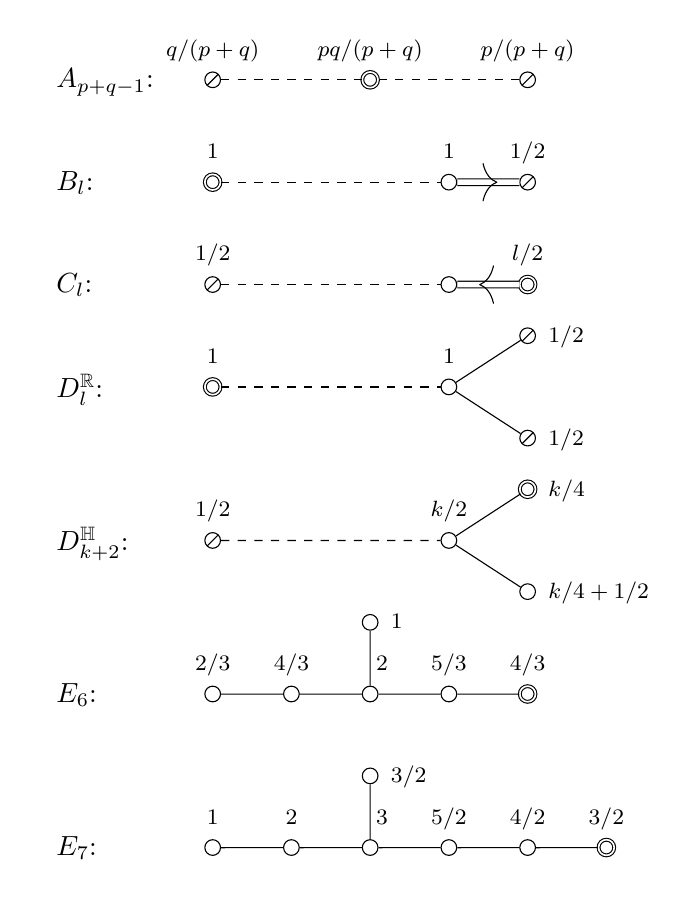
\begin{tikzpicture}[
  yscale=-1.3,
  every node/.style={draw,circle,inner sep=2pt},
  special/.style={double},
  symplectic/.style={forbidden sign},
  every label/.append style={rectangle,font=\footnotesize,
   inner sep=1ex,text depth=1pt},
  decoration={markings,mark=at position 0.7 with {\arrow{>}}},
  doubledynkin/.style={double distance=2pt,postaction=decorate}
  ]
  \node[draw=none] (Atext) [label=right:{\normalsize$A_{p+q-1}$:}] at (-1.25,0) {};
  \node[symplectic] (A1) [label={$q/(p+q)$}] at (1,0) {};
  \node[special] (Ap) [label={$pq/(p+q)$}] at (3,0) {};
  \node[symplectic] (Ak) [label={$p/(p+q)$}] at (5,0) {};
  \draw[dashed] (A1) -- (Ap);
  \draw[dashed] (Ap) -- (Ak);

  \node[draw=none] (Btext) [label=right:{\normalsize$B_{l}$:}] at (-1.25,1) {};
  \node[special] (B1) [label={$1$}] at (1,1) {};
  \node (Blm1) [label={$1$}] at (4,1) {};
  \node[symplectic] (Bl) [label={$1/2$}] at (5,1) {};
  \draw[dashed] (B1) -- (Blm1);
  \draw[doubledynkin] (Blm1) -- (Bl);

  \node[draw=none] (Ctext) [label=right:{\normalsize$C_{l}$:}] at (-1.25,2) {};
  \node[symplectic] (C1) [label={$1/2$}] at (1,2) {};
  \node (Clm1) at (4,2) {};
  \node[special] (Cl) [label={$l/2$}] at (5,2) {};
  \draw[dashed] (C1) -- (Clm1);
  \draw[doubledynkin] (Cl) -- (Clm1);

  \node[draw=none] (DRtext) [label=right:{\normalsize$D_{l}^{\RR}$:}] at (-1.25,3) {};
  \node[special] (DR1) [label={$1$}] at (1,3) {};
  \node (DRlm2) [label={$1$}] at (4,3) {};
  \node[symplectic] (DRlm1) [label=right:{$1/2$}] at (5,2.5) {};
  \node[symplectic] (DRl) [label=right:{$1/2$}] at (5,3.5) {};
  \draw[dashed] (DR1) -- (DRlm2);
  \draw (DRlm1) -- (DRlm2) -- (DRl);

  \begin{scope}[yshift=0.5cm]
   \node[draw=none] (DRtext) [label=right:{\normalsize$D_{k+2}^{\HQ}$:}] at (-1.25,4) {};
   \node[symplectic] (DR1) [label={$1/2$}] at (1,4) {};
   \node (DRlm2) [label={$k/2$}] at (4,4) {};
   \node[special] (DRlm1) [label=right:{$k/4$}] at (5,3.5) {};
   \node (DRl) [label=right:{$k/4+1/2$}] at (5,4.5) {};
   \draw[dashed] (DR1) -- (DRlm2);
   \draw (DRlm1) -- (DRlm2) -- (DRl);
  \end{scope}

  \node[draw=none] (DRtext) [label=right:{\normalsize$E_6$:}] at (-1.25,6) {};
  \node (E61) [label={$2/3$}] at (1,6) {};
  \node (E62) [label={$4/3$}] at (2,6) {};
  \node (E63) [label={\hbox{\hss\quad$2$}}] at (3,6) {};
  \node (E64) [label=right:{$1$}] at (3,5.3) {};
  \node (E65) [label={$5/3$}] at (4,6) {};
  \node[special] (E66) [label={$4/3$}] at (5,6) {};
  \draw (E61) -- (E62) -- (E63) -- (E64);
  \draw (E63) -- (E65) -- (E66);

  \begin{scope}[yshift=0.5cm]
   \node[draw=none] (DRtext) [label=right:{\normalsize$E_7$:}] at (-1.25,7) {};
   \node (E71) [label={$1$}] at (1,7) {};
   \node (E72) [label={$2$}] at (2,7) {};
   \node (E73) [label={\hbox{\hss\quad$3$}}] at (3,7) {};
   \node (E74) [label=right:{$3/2$}] at (3,6.3) {};
   \node (E75) [label={$5/2$}] at (4,7) {};
   \node (E76) [label={$4/2$}] at (5,7) {};
   \node[special] (E77) [label={$3/2$}] at (6,7) {};
   \draw (E71) -- (E72) -- (E73) -- (E74);
   \draw (E73) -- (E75) -- (E76) -- (E77);
  \end{scope}
 \end{tikzpicture}
\]
\end{minipage}\hfill% -}}}3
\newdimen\curparindent
\curparindent=\parindent
\begin{minipage}{.41\textwidth} % {{{-3
 \parindent=\curparindent
 \divide\parindent by 3
 \multiply\parindent by 2
 \noindent
 \small
Legend (and comparison with \cite{Del_ShimVar}):
\begin{itemize}[leftmargin=\parindent]
 \item nodes are represented by circles~%
  \tikz \node[draw,circle,inner sep=2pt] {};
  (bars in \cite{Del_ShimVar});
 \item special nodes are represented by double circles~%
  \tikz \node[draw,circle,inner sep=2pt,double] {};
  (circled nodes in \cite{Del_ShimVar});
 \item symplectic nodes (defined below) are represented by slashed circles~%
  \tikz \node[draw,circle,inner sep=2pt,forbidden sign] {};
  (underlined nodes in \cite{Del_ShimVar}).
\end{itemize}

The number next to a node $\omega$ is $\langle \mu,\omega \rangle$,
where $\mu$ is the cocharacter corresponding to the special node,
and $\omega$ is identified with the appropriate character.

In diagram~$A_{p+q-1}$ it is the $p$-th node that is special.
The diagram~$D_{k+2}^{\HQ}$ is required to satisfy $k + 2 \ge 5$.

The diagrams of type~$E_8$, $F_4$, and~$G_2$ do not occur:
they do not have special nodes.
The diagrams of type~$E_6$ and~$E_7$ do not have symplectic nodes.
\end{minipage} % -}}}3

\paragraph{} % {{{-2
\label{opposition-involution}
We recall the definition of the opposition involution on a Dynkin diagram.
Let $(R,\Phi)$ be an irreducible root system, and
let $\Delta \subset \Phi$ be a choice of positive simple roots.
Then $\Delta$ may be identified with
the vertices of the Dynkin diagram of~$(R,\Phi)$.
Let $W$ be the Weyl group of~$(R,\Phi)$, and
let $w_0$ be the longest element of the Weyl group (with respect to~$\Delta$).
Then $w_0(\Delta) = -\Delta$
and $-w_0$ defines an element~$\tau$ of $\Aut(\Delta)$:
the \emph{opposition involution}.
This involution is non-trivial if and only if
$\Delta$ has type $A_k$ with $k \ne 1$, $D_k$ with $k$~odd, or $E_6$.

For Dynkin diagrams with multiple connected components
the opposition involution is defined as the disjoint union
of the componentwise opposition involutions.

\begin{definition} % {{{-2
 \label{symplectic-node}
	Let $\Delta$ be a connected Dynkin diagram with opposition involution~$\tau$,
 and let $\mu \in \Delta$ be a special node.
 A node $\omega \in \Delta$ is called a \emph{symplectic} node
 (with respect to~$\mu$)
 if $\langle \mu, \omega + \tau(\omega) \rangle = 1$.
\end{definition}

\paragraph{} % {{{-2
The reasoning behind this terminology is best understood
in terms of Deligne's construction
(\cref{delignes-construction}, see also \S1.3 and~\S2.3 of~\cite{Del_ShimVar}):
the symplectic nodes correspond precisely to
the highest weights of symplectic representations~$V$
such that $\mu$ defines a $\{-1,0,1\}$-grading on~$V$.

\begin{definition} % {{{-2
 \label{symplectic-nodes-deligne-dynkin-diagram}
 Let $\Delta^{\mu}$ be a Deligne--Dynkin diagram over a field~$Q$.
 The \emph{subset of symplectic nodes} attached to $\Delta^{\mu}$
 is the maximal subset $S \subset \Delta$ defined by the following conditions:
 \begin{enumerate}
  \item For every special node $\alpha \in \mu \subset \Delta$,
   let $\Delta_\alpha$ denote the connected component of~$\Delta$
   that contains~$\alpha$.
   Then $S \cap \Delta_\alpha$ consists only of
   symplectic nodes of~$\Delta_\alpha$ with respect to~$\alpha$.
   (See also \cref{table-deligne-dynkin-diagrams}.)
  \item The set $S$ is stable under the action of $\Gal(\bar Q/Q)$.
 \end{enumerate}
\end{definition}

\begin{definition} % {{{-2
 A Deligne--Dynkin diagram $\Delta^{\mu}$ over~$Q$ is \emph{symplectic}
 if for every irreducible component of $\Delta^{\mu}$
 its subset of symplectic nodes is non-empty.
\end{definition}

\begin{theorem} % {{{-2
 \label{deldyn-symplectic}
 If $M$ is a hyperadjoint abelian motive over a field $K \subset \CC$,
 then the Deligne--Dynkin diagram $\Delta^{\mu}$
 associated with~$M$ is symplectic.
 \begin{proof}
  Since $M$ is an abelian motive,
  there is an abelian variety $A/K$ such that $M \in \Tangen{\HH^1(A)}$.
  Therefore there is a quotient map $\GB(A) \onto \GB(M)$,
  and hence a map $\tilde\GG_{\mathrm{B}}(M) \to \GB(A)^{\der}$,
  where $\tilde\GG_{\mathrm{B}}(M)$ denotes
  the simply-connected cover of~$\GB(M)$.
  The representation $\GB(A) \to \GL(\HB^1(A))$ is symplectic,
  and thus its restriction to $\tilde\GG_{\mathrm{B}}(M)$ is symplectic.
  In \S1.3 and~\S2.3.7 of~\cite{Del_ShimVar}, Deligne shows that this means
  that $\Delta^{\mu}$ is symplectic.
 \end{proof}
\end{theorem}

\paragraph{The type of $\Delta^\mu$} % {{{-2
Let $\Delta^{\mu}$ be an irreducible populated Deligne--Dynkin diagram over~$Q$.
If $\Delta^{\mu}$ is symplectic,
the type of its connected components is classical:
$A_n$,~$B_n$, $C_n$, or~$D_n$.
Conversely, if the connected components of~$\Delta$
are of type $A_n$ (resp.~$B_n$, or~$C_n$),
then $\Delta^{\mu}$ is symplectic.
In this case we say that the \emph{type} of~$\Delta$
is $A_n$ (resp.~$B_n$ or~$C_n$).
The case where the connected components of~$\Delta$
are of type~$D_n$ requires more attention.

Assume that the connected components of~$\Delta$
are of type~$D_n$, with $n \ge 5$.
For every special node $\alpha \in \mu \subset \Delta$,
let $\Delta_\alpha$ be the connected component of~$\Delta$
that contains~$\alpha$.
The pair $(\Delta_\alpha, \alpha)$ is of type~$D_n^\RR$ or~$D_n^\HQ$
according to the diagrams listed in \cref{table-deligne-dynkin-diagrams}.
One readily verifies that $\Delta^{\mu}$ is symplectic if and only if
one of the following conditions holds:
\begin{itemize}
 \item for every special node~$\alpha$, the pair $(\Delta_\alpha, \alpha)$
  is of type $D_n^\RR$; or
 \item for every special node~$\alpha$, the pair $(\Delta_\alpha, \alpha)$
  is of type $D_n^\HQ$.
\end{itemize}
We say that $\Delta^\mu$ is of \emph{type}~$D_n^\RR$ (resp.~$D_n^\HQ$)
if the former (resp.~the latter) condition holds.

Now assume that the connected components of~$\Delta$ are of type~$D_4$.
Let $V$ be the subset of extremal nodes of~$\Delta$,
let $\bar\mu$ be the $\Gal(\bar Q/Q)$-closure of~$\mu$,
and let $S$ be the subset of symplectic nodes of $\Delta^{\mu}$.
Observe that $S \subset V$,
and $S$ meets every compontent of~$\Delta$ in $0$,~$1$, or~$2$ nodes.
(In other words, the degree of~$S$ over $\pi_0(\Delta)$ is at most~$2$.)
In the first case, $S$ is empty, and $\Delta^{\mu}$ is not symplectic.
In the latter two cases $V = \bar\mu \sqcup S$, by the maximality of~$S$.
We say that $\Delta^{\mu}$ has \emph{type} $D_4^\RR$
if $\deg(\bar\mu) = 1$ and $\deg(S) = 2$,
while $\Delta^{\mu}$ has \emph{type} $D_4^\HQ$
if $\deg(\bar\mu) = 2$ and $\deg(S) = 1$.

\begin{remark} % {{{-2
 \label{type-remarks}
 Let $Q'/Q$ be a field extension,
 and let $\Delta^{\mu}$ be a Deligne--Dynkin diagram over~$Q$.
 By restricting the Galois action,
 one obtains a Deligne--Dynkin diagram $\Delta^{\mu}_{Q'}$ over~$Q'$.
 We make the following observations:
 \begin{enumerate}
  \item If $\Delta^{\mu}$ is irreducible or populated
   then this need not be true for $\Delta^{\mu}_{Q'}$.
   (Of course $\Delta^\mu_{Q'}$ will have
   irreducible components that are populated.)
  \item Related to the preceding point:
   the subset of symplectic nodes of $\Delta^{\mu}_{Q'}$
   may be strictly larger than the subset of symplectic nodes of $\Delta^{\mu}$.
  \item If $\Delta^{\mu}$ is irreducible of type~$D_4^\HQ$
   then $\Delta^{\mu}_{Q'}$ may have irreducible components of type~$D_4^\RR$.
   On the other hand, if $\Delta^{\mu}$ is populated and symplectic,
   but not of type~$D_4^\HQ$,
   then every irreducible component of $\Delta^{\mu}_{Q'}$ that is populated
   must have the same type as $\Delta^{\mu}$.
 \end{enumerate}
\end{remark}

\begin{lemma} % {{{-2
 \label{locally-same-type}
 Let $\Delta^{\mu}$ be
 an irreducible symplectic populated Deligne--Dynkin diagram over~$\QQ$.
 Then there exists a prime number~$\ell$,
 and an irreducible component of $\Delta^{\mu}_{\QQl}$
 that has the same type as $\Delta^{\mu}$.
 \begin{proof}
  This is trivial, unless $\Delta^{\mu}$ has type~$D_4^\HQ$.
  In that case, let $\alpha \in \mu$ be a special node,
  and let $\Delta_\alpha$ be
  the connected component of~$\Delta$ that contains~$\alpha$.
  By assumption, the subset of symplectic nodes of $\Delta^{\mu}$
  meets $\Delta_\alpha$ in exactly one node~$s$.
  Label the remaining extremal node of~$\Delta_\alpha$ with $\beta$.
  By assumption we have $\bar\mu \cap \Delta_\alpha = \{\alpha,\beta\}$.
  By Chebotarev's density theorem
  there exists a prime number~$\ell$
  and an element $g \in \Gal(\QQlbar/\QQl)$ such that $g\alpha = \beta$.
  Let $\Delta'$ be the $\Gal(\QQlbar/\QQl)$-closure of $\Delta_\alpha$,
  and take $\mu' = \Delta' \cap \mu$.
  Then $(\Delta', \mu')$ has type~$D_4^\HQ$.
 \end{proof}
\end{lemma}

\paragraph{} % {{{-2
An \emph{isomorphism of Deligne--Dynkin diagrams}
$\phi \colon \Delta_1^{\mu_1} \to \Delta_2^{\mu_2}$ over a field~$Q$
is a $\Gal(\bar Q/Q)$-equivariant isomorphism
$\phi \colon \Delta_1 \to \Delta_2$ that maps $\mu_1$ onto~$\mu_2$.

Observe that there is a natural map
$\Isom(\Delta_1^{\mu_1},\Delta_2^{\mu_2})
\to \Isom(\pi_0(\Delta_1),\pi_0(\Delta_2))$,
and if $f \in \Isom(\pi_0(\Delta_1),\pi_0(\Delta_2))$,
then we write $\Isom_f(\Delta_1^{\mu_1},\Delta_2^{\mu_2})$
for the set of $\phi \in \Isom(\Delta_1^{\mu_1},\Delta_2^{\mu_2})$
such that $\pi_0(\phi) = f$.

\begin{lemma} % {{{-2
 Let $\Delta^{\mu}$ be
 an irreducible symplectic populated Deligne--Dynkin diagram over~$Q$.
 Let $\tau$ denote the opposition involution on~$\Delta$.
 Then
 \[
  \#\Aut_\id(\Delta^\mu) =
  \begin{cases}
   1 &\text{if $\Delta^\mu$ has type $A_1$,~$B_n$, $C_n$, $D_n^\HQ$,
   or $A_n$ and $\mu$ is not fixed by~$\tau$,}\\
   2 &\text{if $\Delta^\mu$ has type $D_n^\RR$, or $A_n$ ($n \ge 2$)
    and $\mu$ is fixed by~$\tau$.}
  \end{cases}
 \]
\end{lemma}

\begin{lemma} % {{{-2
 \label{locally-same-aut}
 Let $\Delta^{\mu}$ be
 an irreducible symplectic populated Deligne--Dynkin diagram over~$\QQ$.
 Then there exists
 an irreducible component $\Delta_\lambda^{\mu_\lambda}$ of $\Delta^{\mu}_{\QQl}$
 such that the natural map
 $\Aut_\id(\Delta^\mu) \to \Aut_\id(\Delta_\lambda^{\mu_\lambda})$
 is an isomorphism.
 \begin{proof}
  This follows immediately from \cref{locally-same-type}.
 \end{proof}
\end{lemma}

\paragraph{} % {{{-2
\label{deg2-set}
Let $\Delta^{\mu}$ be
an irreducible symplectic populated Deligne--Dynkin diagram over~$Q$.
The action of $\Gal(\bar Q/Q)$ on~$\Delta$
is determined by the action on
a $\Gal(\bar Q/Q)$-closed subset $U(\Delta^\mu)$ of~$\Delta$.
Let $S$ be the subset of symplectic nodes of~$\Delta^\mu$.
\begin{itemize}
 \item If $\Delta^\mu$ is of type~$A_n$, we take~$U(\Delta^\mu) = S$.
 \item If $\Delta^\mu$ is of type~$B_n$, we take $U(\Delta^\mu) = S$.
 \item If $\Delta^\mu$ is of type~$C_n$, we take $U(\Delta^\mu) = \bar\mu$.
 \item If $\Delta^\mu$ is of type~$D_n^\RR$, we take $U(\Delta^\mu) = S$.
 \item If $\Delta^\mu$ is of type~$D_n^\HQ$,
  we take $U(\Delta^\mu) = \bar\mu$.
\end{itemize}
Note that the degree of $U(\Delta^\mu)$ over~$\pi_0(\Delta)$ is at most~$2$.

\paragraph{} % {{{-2
Let $\Delta_1^{\mu_1}$ and~$\Delta_2^{\mu_2}$ be two
irreducible symplectic populated Deligne--Dynkin diagrams over~$\QQ$.
Suppose there is a $\phi \in \Isom_f(\Delta_1^{\mu_1},\Delta_2^{\mu_2})$,
where $f$ is some $\Gal(\QQbar/\QQ)$-equivariant isomorphism
$\pi_0(\Delta_1) \to \pi_0(\Delta_2)$.
Let $\ell$ be a prime number.
Identify $\pi_0(\Delta_1)$ with $\Hom(E,\QQbar)$
for some number field~$E$.

We restrict the Galois action to $\Gal(\QQlbar/\QQl)$.
The irreducible components of~$(\Delta_1^{\mu_1})_{\QQl}$
are in a natural way indexed by the places~$\lambda$ of~$E$
that lie above~$\ell$.
In a similar manner, the maps~$f_\ell$ and~$\phi_\ell$
are the disjoint union of local components~$f_\lambda$ and~$\phi_\lambda$.
We will use this notation below.

\begin{proposition} % {{{-2
 \label{deldyn-local-global}
 Let $\Delta_1^{\mu_1}$ and~$\Delta_2^{\mu_2}$ be two
 irreducible symplectic populated Deligne--Dynkin diagrams over~$\QQ$.
 Suppose that there is an isomorphism
 $f \colon \pi_0(\Delta_1) \to \pi_0(\Delta_2)$
 and for each prime number~$\ell$ an element
 $\psi_\ell \in \Isom_f(\Delta_{1,\QQl}^{\mu_1},\Delta_{2,\QQl}^{\mu_2})$.
 Let $E$ be a number field such that $\Hom(E,\QQbar) = \pi_0(\Delta_1)$.

 Then there exists a $\phi \in \Isom_f(\Delta_1^{\mu_1},\Delta_2^{\mu_2})$
 and a finite place~$\lambda$ of~$E$
 such that $\phi_\lambda = \psi_\lambda$.
 \begin{proof}
  It suffices to prove the existence of~$\phi$;
  the second claim will follow automatically from \cref{locally-same-aut}.
  First of all, observe that $\Delta_1^{\mu_1}$ and~$\Delta_2^{\mu_2}$
  must have the same type, by \cref{type-remarks} and \cref{locally-same-type}.
  Next, we claim that there is an element in
  $\Isom_f(U(\Delta_1^{\mu_1}),U(\Delta_2^{\mu_2}))$.
  Indeed, since the degree of~$U(\Delta_i^{\mu_i})$ over~$\pi_0(\Delta_i)$
  is at most~$2$,
  it suffices (by Chebotarev's density theorem)
  to prove that these sets are locally isomorphic.
  If the type is not~$D_4^\HQ$,
  such local isomorphisms are obtained
  by restricting the~$\psi_\ell$ to~$U(\Delta_1^{\mu_1})$.
  If the type is~$D_4^\HQ$,
  all $\psi_\ell$ will map $\mu_1$ to~$\mu_2$,
  but they need not all map $\Gal(\QQbar/\QQ)\cdot\mu_1$
  to~$\Gal(\QQbar/\QQ)\cdot\mu_2$.
  Suppose that $\psi_\lambda$ is a component of some~$\psi_\ell$
  that does not map $(\Gal(\QQbar/\QQ)\cdot\mu_1) \cap \Delta_{1,\lambda}$
  to $(\Gal(\QQbar/\QQ)\cdot\mu_2) \cap \Delta_{2,\lambda}$.
  In that case the vertices of $\Delta_{i,\lambda}$
  form $4$~orbits under $\Gal(\QQlbar/\QQl)$
  and in particular there is an element in
  $\Isom_{f_\lambda}(U(\Delta_1^{\mu_1})_{\lambda},
  U(\Delta_2^{\mu_2})_{\lambda})$.
  This proves the claim that
  $\Isom_f(U(\Delta_1^{\mu_1}),U(\Delta_2^{\mu_2}))$ is non-empty.
  As a consequence there is an element
  $\phi \in \Isom_f(\Delta_1, \Delta_2)$ (see~\cref{deg2-set}).

  It remains to prove that we can choose~$\phi$
  in such a way that it maps $\mu_1$ to~$\mu_2$.
  If $\Delta_1^{\mu_1}$ and $\Delta_2^{\mu_2}$
  are of type $A_1$,~$B_n$, $C_n$, or~$D_n^\RR$ ($n \ge 5$),
  then the topology of the diagram forces $\phi(\mu_1) = \mu_2$,
  hence there is nothing left to do.
  Now suppose that the type is $A_n$, with $n \ge 2$.
  If $\mu_1$ (and therefore $\mu_2$) is fixed
  under the opposition involution,
  then there is again nothing to do.
  If the type is $D_4^\RR$,
  recall that $U(\Delta_i^{\mu_i}) = S_i$,
  so we can choose $\phi$ such that $\phi(S_1) = S_2$.
  This means that $\phi(\bar\mu_1) = \bar\mu_2$,
  and we conclude that $\phi(\mu_1) = \mu_2$.

  Finally, suppose that the type is $D_n^\HQ$,
  or the type is $A_n$ and $\mu_i$ is not fixed by the opposition involution.
  Let $S_i$ be the subset of symplectic nodes of~$\Delta_i^{\mu_i}$,
  and observe that $\phi(S_1) = S_2$.
  There is a unique non-trivial involution~$\tau_i \in \Aut_\id(\Delta_i)$
  such that $\tau_i(S_i) = S_i$.
  Now remark that $\phi \circ \tau_1 = \tau_2 \circ \phi$.
  Let $\alpha \in \mu_1$ be a special node that is not fixed under~$\tau_1$.
  We may assume that $\phi(\alpha) \in \mu_2$,
  by replacing $\phi$ with $\phi \circ \tau_1$ if necessary.
  
  We claim that $\phi(\mu_1) = \mu_2$.
  Indeed, suppose that $\alpha' \in \mu_1$ is a special node, and
  let $\Delta_{\alpha'}$ be the component of~$\Delta_1$ containing~$\alpha'$.
  There exists a $g \in \Gal(\QQbar/\QQ)$ such that
  \[
   \begin{cases}
    g\alpha = \alpha' &\text{if the type is~$D_4^\HQ$}\\
    g\alpha \in \Delta_{\alpha'} &\text{otherwise.}
   \end{cases}
  \]
  By Chebotarev's density theorem,
  we may assume that $g \in \Gal(\QQlbar/\QQl)$
  for some prime number~$\ell$.

  If the type is $D_4^\HQ$, then
  \[
   \phi(\alpha') = \phi(g\alpha) = g\phi(\alpha) = g\psi_\ell(\alpha)
   = \psi_\ell(g\alpha) = \psi_\ell(\alpha') \in \mu_2.
  \]
  Finally, if the type is not~$D_4^\HQ$, then we argue as follows:
  Let $\Delta_{1,\lambda}^{\mu_{1,\lambda}}$
  (resp.~$\Delta_{2,\lambda}^{\mu_{2,\lambda}}$)
  be the irreducible component of~$\Delta_{1,\QQl}^{\mu_1}$
  (resp.\ $\Delta_{2,\QQl}^{\mu_2}$)
  that contains~$\alpha$ (resp.~$\phi(\alpha)$).
  It is clear that $\phi_\lambda = \psi_\lambda$,
  and hence $\phi(\alpha') \in \mu_2$.
  This concludes the proof.
 \end{proof}
\end{proposition}

\paragraph{} % {{{-2
Let $M$ be a hyperadjoint abelian motive
over a finitely generated field $K \subset \CC$.
Let $\Delta^\mu$ be the Deligne--Dynkin diagram associated with~$M$.
Choose an embedding of $K$ into a $p$-adic field~$K_v$.
Let $C_v$ be the completion of an algebraic closure of~$K_v$.
By $p$-adic Hodge theory,
we know that there is a grading on $\Hp(M) \otimes_{\QQp} C_v$.
This determines a cocharacter~$\mu_{\HT}$ of
$\Gpc(M) \otimes_{\QQp} C_v \subset \GB(M) \otimes_\QQ C_v$,
the \emph{Hodge--Tate} cocharacter.

\begin{lemma} % {{{-2
 \label{hodge-tate-cochar-deldyn}
 Retain the notation of the preceding paragraph.
 The conjugacy class of the cocharacter
 $\mu_{\HT} \colon \Gm[C_v] \to \GB(M) \otimes_\QQ C_v$
 is defined over~$\QQbar$ and coincides with the
 conjugacy class of the Hodge cocharacter
 $\mu \colon \Gm[\CC] \to \GB(M) \otimes_\QQ \CC$.
 In particular, $\mu_{\HT}$ determines the subset $\mu \subset \Delta$.
 \begin{proof}
  This follows from the comparison theorems
  between Betti cohomology, algebraic de~Rham cohomology,
  and $p$-adic \'etale cohomology.
 \end{proof}
\end{lemma}

\section{Deligne's construction} % {{{-1
\label{delignes-construction}

\readme % {{{-2
Let $M$ be an irreducible hyperadjoint abelian motive over~$\CC$.
Proposition~2.3.10 of~\cite{Del_ShimVar} provides a recipe
to construct a complex abelian variety~$A$ (up to isogeny)
such that $M \cong \HH^1(A)^\ha$.
Deligne uses the language of Shimura data and Hodge theory.
We recall this construction,
using the terminology of abelian motives and Deligne--Dynkin diagrams.

\paragraph{Preparations} % {{{-2
Let $M$ be an irreducible hyperadjoint abelian motive over~$\CC$.
Let $E$ denote $\End(M)$,
and let $\Delta^{\mu}$ be the Deligne--Dynkin diagram associated with~$M$.
Recall that $E$ is a totally real field
(see the discussion in~\S2.3.4(a) of~\cite{Del_ShimVar}),
and note that $\Hom(E,\QQbar) \cong \pi_0(\Delta)$.
We also recall that $\Delta^{\mu}$ is symplectic (\cref{deldyn-symplectic}).
Let $S$ be the subset of symplectic nodes of~$\Delta^{\mu}$.

Write $G$ for the $\QQ$-simple adjoint group $\GB(M)$,
and let $\tilde G$ be the simply-connected cover of~$G$.
For $s \in S$, let $V(s)$ be the representation of~$\tilde G_\CC$
whose highest weight corresponds to~$s$.
Since $S$ is closed under the action of~$\Gal(\QQbar/\QQ)$,
there exists a representation~$V$ of~$\tilde G$ over~$\QQ$
such that $V_\CC \cong \bigoplus_{s \in S} V(s)^{\oplus n}$
for suitable~$n$.

\paragraph{Choices} % {{{-2
\label{choices}
Now we fix three choices:
\begin{enumerate}
 \item Choose a totally imaginary quadratic extension $F/E$.
 \item Choose a partial \cm~type~$\Phi$ for~$F$ relative to $\Delta^\mu$:
  a subset $\Phi \subset \Hom(F,\CC) = \Hom(F,\QQbar)$
  that maps 1-to-1 onto the complement of the image of~$\mu$
  in $\Hom(E,\QQbar) = \pi_0(\Delta)$.
 \item Choose a representation~$V$ of~$\tilde G$ as above.
\end{enumerate}

\paragraph{} % {{{-2
The Hodge cocharacter $h \colon \DelS \to G_\RR$ lifts to a map
$\tilde h \colon \tilde \DelS \to \tilde G_\RR$,
endowing~$V$ with a fractional Hodge structure.
The Hodge decomposition of~$V$ may be read off from
the diagrams in~\cref{table-deligne-dynkin-diagrams}.
If $s \in S$ lies in a component of~$\Delta$ that does not meet~$\mu$,
then the type of~$V(s)$ is $\{(0,0)\}$.
If $s$ lies in a component of~$\Delta$
that contains a special node $\alpha \in \mu$,
then the type of~$V(s)$ is $\{(r,-r), (r-1, 1-r)\}$
where $r = \langle s, \alpha \rangle$ is the number
that is written next to the node~$s$
in the appropriate diagram in~\cref{table-deligne-dynkin-diagrams}.

\paragraph{} % {{{-2
Let $F_S$ denote the \'etale $E$-algebra
such that $\Hom(F_S, \QQbar) \cong S$ as $\Gal(\QQbar/\QQ)$-sets.
Observe that the fractional Hodge structure~$V$
is canonically an $F_S$-module:
the algebra~$F_S$ acts on~$V(s)$
via the embedding $F_S \into \QQbar \subset \CC$
that corresponds with $s \in S$.

We endow $F_S$ with a fractional pre-Hodge structure:
the component $\CC^{\{s\}}$ of $F_S \otimes_\QQ \CC \cong \CC^S$
is placed in bi-degree $(0,0)$
if $s$ lies in a component of~$\Delta$ that does not meet~$\mu$;
and $\CC^{\{s\}}$ is placed in bi-degree $(1-r,r)$
if $s$ lies in a component that does meet~$\mu$,
where $r$ is the rational number from the preceding paragraph.

In a similar fashion we endow the \cm~field~$F$ with
a fractional pre-Hodge structure:
the component $\CC^\phi$ of $F \otimes \CC \cong \CC^{\Hom(F,\CC)}$
is placed in bi-degree
\[
 \begin{cases}
  (1,0) &\text{if $\phi \in \Phi$}\\ %TODO is this the right convention?
  (0,1) &\text{if $\bar\phi \in \Phi$}\\
  (0,0) &\text{otherwise.}
 \end{cases}
\]

\paragraph{} % {{{-2
\label{WF}
Write $W_F$ for $F \otimes_E F_S$, and
observe that $F \otimes_E F_S$ is a fractional Hodge structure of weight~$1$.
Note that $W_F$ is of \cm~type,
since both~$F$ and $F_S$ are of \cm~type.
Put $V' = W_F \otimes_{F_S} V$.
A computation shows that $V'$
is a Hodge structure of type $\{(1,0), (0,1)\}$.
It turns out that $V'$~is a polarisable Hodge structure
(see \cite{Del_ShimVar} for details).
Thus there is a complex abelian variety~$A$ (well-defined up to isogeny)
such that $\HB^1(A) \cong V'$.
Since $W_F$ is of \cm~type,
we find that $\GB(V')^\ad = G$,
and therefore $\HH^1(A)^\ha = M$.

\paragraph{} % {{{-2
\label{tori-isog}
Write $T$ for the torus $\GB(A)^\ab = \GB(V')^\ab$.
Choose a faithful representation~$N$ of~$T$;
by the Tannakian formalism and \cref{hodge-is-motivated}
we may view~$N$ as an abelian \cm~motive over~$\CC$.

Since $\GB(W_F)$ is a torus, and $\tilde G$ is almost simple,
the representation
\[
 \GB(W_F) \times \tilde G \to \GL(V') = \GL(W_F \otimes_{F_S} V)
\]
has a finite kernel.
In other words, the natural map
$\GB(W_F) \times \tilde G \to \GB(A)$ is an isogeny,
and so is the natural map $\GB(W_F) \to T$.

% \paragraph{} % {{{-2
% We end this section with a picture of the $\ell$-adic side of this story.
% Let $K \subset \CC$ be a finitely generated field
% such that the motive~$M$ and the abelian variety~$A$ are defined over~$K$.
% We have the following diagram:
% \[
%  \begin{tikzpicture}[commutative diagrams/every diagram]
%   \node (Gal) at (-4,-1.75) {$\Gal(\bar K/K)$};
%   \node (GlA) at (0,0) {$\Gl(A)$};
%   \node (GlMt) at (90:1.7) {$\widetilde{\Gl(M)}$};
%   \node (GlN) at (55:-1.7) {$\Gl(N)$};
%   \node (GlM) at (110:-2) {$\Gl(M)$};
%   \node (HlA) at ($(0,0) +(5,0)$) {$\GL(\Hl(A))$};
%   \node (HlN) at ($(55:-1.7) +(5,0)$) {\GL($\Hl(N))$};
%   \node (HlM) at ($(110:-2) +(5,0)$) {$\GL(\Hl(M))$};
%   \path[commutative diagrams/.cd, every arrow, every label]
%   (GlM) edge (HlM)
%   (GlN) edge (HlN)
%   (GlA) edge (HlA)
%   (GlMt) edge (GlA)
%   (GlA) edge [commutative diagrams/crossing over] (GlM)
%   (GlA) edge (GlN)
%   (Gal) edge (GlA)
%   (Gal) edge (GlN)
%   (Gal) edge (GlM);
%  \end{tikzpicture}
% \]
% Indeed, the map from $\Gal(\bar K/K)$ to $\Gl(A)$
% exists by our assumption that $A$ is defined over~$K$.

\section{The main proposition} % {{{-1

\readme % {{{-2
In this section we prove the main technical result of this paper.
Its proof uses results of the preceding three sections.

\begin{proposition} % {{{-2
 \label{mtc-product-abelian-motives}
 Let $M_1$ and~$M_2$ be two
 geometrically irreducible hyperadjoint abelian motives
 over a finitely generated field $K \subset \CC$.
 Assume that $\MTC(M_1)$ and $\MTC(M_2)$ are true, and
 assume that $\Gl(M_1 \oplus M_2)$ is connected for all prime numbers~$\ell$.
 If there exists a prime number~$\ell$
 such that $\Gl(M_1 \oplus M_2) \subsetneq \Gl(M_1) \times \Gl(M_2)$,
 then $\HB(M_1) \cong \HB(M_2)$ as Hodge structures.
\end{proposition}

\paragraph{} % {{{-2
\label{prp-strategy}
The proof of this \namecref{mtc-product-abelian-motives}
will take the rest of this section.
The strategy is as follows:
\begin{enumerate}
 \item First we prove that $\End(M_1) = \End(M_2)$.
 \item Next we show that $\Hl(M_1) \cong \Hl(M_2)$ for all primes~$\ell$.
 \item We use this (and \cref{deldyn-local-global})
  to show that $M_1$ and~$M_2$
  have isomorphic Deligne--Dynkin diagrams over~$\QQ$.
 \item After that we run Deligne's construction (\cref{delignes-construction})
  on the motives~$M_i$;
  this leaves us with two complex abelian varieties~$A_1$ and~$A_2$
  such that $M_{i,\CC} = \HH^1(A_i)^\ha$.
 \item We replace $K$ be a finitely generated extension,
  such that $A_1$ and~$A_2$ are defined over~$K$.
 \item By carefully tracing the $\ell$-adic counterpart of the construction
  we show that $A_1$ and~$A_2$ have isomorphic $\ell$-adic Tate modules.
 \item Finally, we apply Faltings's results to deduce that $A_1$ and~$A_2$
  are isogenous, which implies $\HB(M_1) \cong \HB(M_2)$.
\end{enumerate}
Sadly however, this strategy is slightly too optimistic.
It is not possible to work with the entire $\ell$-adic Galois representations:
we will have to focus our attention on a suitable summand.
This makes the proof quite technical.

\paragraph{} % {{{-2
We first make some observations about~$M_1$ and~$M_2$.
For $i \in \{1,2\}$,
write $E_i$ for $\End(M_i)$, and
write $\Lambda_i$ for the set of finite places of~$E_i$.
For a prime number~$\ell$, let $\Lambda_{i,\ell}$
denote the set of places~$\lambda \in \Lambda_i$ that lie above~$\ell$.
Since $\MTC(M_i)$ holds, we know that %TODO explain
$\Glc(M_i) = \prod_{\lambda \in \Lambda_{i,\ell}}
\Res_{E_{i,\lambda}/\QQl} \Glambdac(M_i)$.
By assumption $\Gl(M_i) = \Glc(M_i)$,
and hence $\Glambda(M_i) = \Glambdac(M_i)$.
We also know that
$\Glambda(M_i)$ is a simple adjoint group over~$E_{i,\lambda}$,
once again, because $\MTC(M_i)$ holds. %TODO explain
Finally, observe that $\HH_{\Lambda_i}(M_i)$ is a
quasi-compatible system of representations,
by \cref{abelian-motive-quasi-compatible-realisations}.

Let $\ell$ be a prime number
such that $\Gl(M_1 \oplus M_2) \subsetneq \Gl(M_1) \times \Gl(M_2)$.
By Goursat's lemma this implies that there are
places $\lambda_1 \in \Lambda_{1,\ell}$
and $\lambda_2 \in \Lambda_{2,\ell}$
such that the projection of $\Gl(M_1 \oplus M_2)$ in
$\Res_{E_{1,\lambda_1}} \GG_{\lambda_1}(M_1) \times
\Res_{E_{2,\lambda_2}} \GG_{\lambda_2}(M_2)$
is the graph of an isomorphism of algebraic groups over~$\QQl$.
Hence there is a $\QQl$-linear isomorphism %TODO explain
$\psi \colon \HH_{\lambda_1}(M_1) \to \HH_{\lambda_2}(M_2)$
of Galois representations of~$K$.

Note that $\psi$ induces an isomorphism
$f \colon \End_{\Gal(\bar{K}/K)}(\HH_{\lambda_1}(M_1)) \to
\End_{\Gal(\bar{K}/K)}(\HH_{\lambda_2}(M_2))$,
and since these endomorphism algebras are commutative,
the isomorphism~$f$ does not depend on~$\psi$.
By \cref{recover-endomorphisms} we recover
$\lambda_i \colon E_i \into E_{i,\lambda_i} =
\End_{\Gal(\bar{K}/K)}(\HH_{\lambda_i}(M_i))$,
and therefore $\psi$ gives a canonical isomorphism
$f \colon E_1 \to E_2$ that identifies $\lambda_1$ with~$\lambda_2$.
Write $E$ for $E_1 = E_2$,
and write $\lambda$ for $\lambda_1 = \lambda_2$.
We conclude that $\Hlambda(M_1) \cong \Hlambda(M_2)$
as $\lambda$-adic Galois representations.

Write $\Lambda$ for the set of finite places of~$E$.
We assumed that $\Gl(M_{1} \oplus M_{2})$
is connected for all prime numbers~$\ell$.
Because $\Hlambda(M_1)$ and $\Hlambda(M_2)$
are semisimple and quasi-compatible,
\cref{quasi-compatible-semisimple-isomorphic}
shows that $\HLambda(M_1)$ and $\HLambda(M_2)$
are isomorphic quasi-compatible systems of representations.
We have now completed the first two steps of the strategy
outlined in \cref{prp-strategy}.

\paragraph{} % {{{-2
For $i = 1,2$, let $\Delta_i^{\mu_i}$
be the Deligne--Dynkin diagram associated with~$M_i$,
as in \cref{abmotdeldyn}.
Let $f \colon \pi_0(\Delta_1) \to \pi_0(\Delta_2)$ be the map,
that is defined by the canonical identifications
$\pi_0(\Delta_i) \cong \Hom(E,\QQbar)$.
Since $\HLambda(M_1)$ and $\HLambda(M_2)$ are isomorphic
as $E$-linear quasi-compatible systems of representations,
we get local isomorphisms
$\psi_\ell \in \Hom_f(\Delta_{1,\QQl},\Delta_{2,\QQl})$.
By \cref{hodge-tate-cochar-deldyn} we have
$\psi_\ell(\mu_1) = \mu_2$ for all~$\ell$.
Thus we may apply \cref{deldyn-local-global}
to obtain an isomorphism $\phi \in \Isom_f(\Delta_1^{\mu_1},\Delta_2^{\mu_2})$,
such that $\psi_\lambda = \phi_\lambda$ for some finite place~$\lambda$ of~$E$.

Let $S_i$ be the subset of symplectic nodes of~$\Delta_i^{\mu_i}$.
We will now apply Deligne's construction (see \cref{delignes-construction})
to the motives~$M_1$ and~$M_2$.
To do so, we have to make three choices, as in \cref{choices}:
\begin{enumerate*}[label=(\textit{\roman*})]
\item choose a totally imaginary quadratic extension $F/E$, and
\item endow it with a partial \cm~type
 relative to $\Delta_1^{\mu_1} \stackrel{\phi}{=} \Delta_2^{\mu_2}$;
 finally,
\item choose the representations~$V_1$ and~$V_2$
 in such a way that they have the same dimension.
\end{enumerate*}
Let $F_{S_i}$ be an \'etale $E$-algebra such that
$\Hom(F_{S_i},\QQbar) \cong S_i$,
and write $W_{F,i}$ for $F \otimes_E F_{S_i}$.
Recall from \cref{WF} that $W_{F,i}$ carries a
fractional Hodge structure of weight~$1$ that is of \cm~type.
The construction produces two complex abelian varieties~$A_1$ and~$A_2$,
such that $\HB(A_i) = W_{F,i} \otimes_{F_{S_i}} V_i$,
and $M_{i,\CC} = \HH^1(A_i)^\ha$.

\paragraph{} % {{{-2
As in \cref{tori-isog}, let $T_i$ denote the torus $\GB(A_i)^\ab$.
Recall that the natural map $\GB(W_{F,i}) \to T_i$ is an isogeny.
The isomorphism~$\phi$ of Deligne--Dynkin diagrams
induces an isomorphism of fractional Hodge structure $W_{F,1} \cong W_{F,2}$.
Therefore there exists a torus~$T$,
together with isogenies $T_i \to T$.
Let $N$ be a faithful representation of~$T$.
By \cref{hodge-is-motivated} and the Tannakian formalism
we view $N$ as a complex motive.
Note that $N$ is an abelian \cm~motive.

Replace~$K$ with a finitely generated extension of~$K$
such that $A_1$,~$A_2$, and the motive~$N$ are defined over~$K$.
We are now ready for the two final steps in~\cref{prp-strategy}.

\paragraph{} % {{{-2
Let $\lambda$ be a finite place of~$E$ such that $\psi_\lambda = \phi_\lambda$,
and let $\ell$ be the residue characteristic of~$\lambda$.
Observe that $E$ acts on $M_i$,~$V_i$, $W_{F,i}$, and~$A_i$.
Let $\rho_i$ denote the Galois representation
$\Gal(\bar K/K) \to \Gl(A_i)(\QQl) \subset \GL(\Hl(A_i))(\QQl)$.
We make a table of all the data that is canonically identified
by $\phi_\lambda = \psi_\lambda$.
\begin{align*}
 \Glambda(M_1) &= \Glambda(M_2)
 &&\text{henceforth~$\Glambda$} \\
 \widetilde{\Glambda(M_1)} &= \widetilde{\Glambda(M_2)}
 &&\text{henceforth~$\widetilde{\Glambda}$} \\
 F_{S_1} \otimes_E E_\lambda &= F_{S_2} \otimes_E E_\lambda
 &&\text{as $E_\lambda$-algebras, henceforth~$F_{S,\lambda}$} \\
 W_{F,1} \otimes_E E_\lambda &= W_{F,2} \otimes_E E_\lambda
 &&\text{as $E_\lambda$-algebras, henceforth~$W_{F,\lambda}$} \\
 V_1 \otimes_E E_\lambda &= V_2 \otimes_E E_\lambda
 &&\text{as $\widetilde{\Glambda}$-representations
  with $F_{S,\lambda}$-action, henceforth~$V_\lambda$} \\
 \Hlambda(A_1) &= \Hlambda(A_2)
 &&\text{as $\widetilde{\Glambda}$-representations
  with $W_{F,\lambda}$-action, henceforth~$\Hlambda$}
\end{align*}
Let $G' \subset \GL_{E_\lambda}(\Hlambda)$ be the algebraic subgroup
generated by the image of $\widetilde{\Glambda}$
and the image of $W_{F,\lambda}^*$.
For $i = 1,2$, let $\rho_{i,\lambda}$ be
the $\lambda$-adic component of~$\rho_i$.
We may view $\rho_{i,\lambda}$ as a Galois representation on~$\Hlambda$,
and it takes values in~$G'(E_\lambda)$.
Observe that $\Glambda$ is the adjoint group of~$G'$,
and denote the projection with $\pi^\ad \colon G' \onto \Glambda$.
We note that $\pi^\ad \circ \rho_{i,\lambda}$ defines the Galois
representation on $\Hlambda(M_i)$,
and thus $\pi^\ad \circ \rho_{1,\lambda} = \pi^\ad \circ \rho_{2,\lambda}$.

\paragraph{} % {{{-2
Recall that we have an isogeny $p_i \colon \Gl(A_i)^\ab \to T_\ell = \Gl(N)$.
Denote the kernel of this isogeny with~$K_i$.
We also have a composition
$\Gl(A_i) \to \Res_{E_\lambda/\QQl}\Glambda(A_i) \into \Res_{E_\lambda/\QQl}G'$,
and therefore a map $\Gl(A_i)^\ab \to (\Res_{E_\lambda/\QQl}G')^\ab$.
Let $K'_i$ be the image of~$K_i$
in~$(\Res_{E_\lambda/\QQl}G')^\ab$ under this map,
and denote with $T'$ the quotient of $(\Res_{E_\lambda/\QQl}G')^\ab$
by the finite group $K'_1 \cdot K'_2$.
Let $\pi^\ab \colon \Res_{E_\lambda/\QQl}G' \onto T'$ be the natural projection.
We claim that $\pi^\ab \circ \rho_{1,\lambda} = \pi^\ab \circ \rho_{2,\lambda}$.

Indeed, observe that $p_i \circ \rho_i$ defines
the Galois representation on~$\Hl(N)$,
which does not depend on~$i = 1,2$, since the motive~$N$ does not depend on~$i$.
If $q$ denotes the natural projection $T_\ell \onto T'$,
then $q \circ p_i \circ \rho_i = \pi^\ab \circ \rho_{i,\lambda}$.
This proves the claim that
$\pi^\ab \circ \rho_{1,\lambda} = \pi^\ab \circ \rho_{2,\lambda}$.

\paragraph{} % {{{-2
We are almost done!
Recall that $T'$ is a quotient of~$(\Res_{E_\lambda/\QQl}G')^\ab$
by a finite group.
Hence the group $\Gamma = \ker(\pi^\ad) \cap \ker(\pi^\ab)$ is
a finite abelian subgroup of $G'(E_\lambda) = (\Res_{E_\lambda/\QQl}G')(\QQl)$.
Define $\xi \colon \Gal(\bar \Gamma/\Gamma) \to G'(E_\lambda)$
via $\xi(g) = \rho_{1,\lambda}(g) \cdot \rho_{2,\lambda}(g)^{-1}$.
This map $\xi$ takes values in~$\Gamma$,
and is a homomorphism since $\Gamma$ is commutative.
We conclude that after replacing $K$ by a finite extension,
the homomorphisms $\rho_{1,\lambda}$ and~$\rho_{2,\lambda}$ are the same.

This means that $\Hlambda(A_1)$ and~$\Hlambda(A_2)$
are isomorphic as $\lambda$-adic Galois representations.
Another application of \cref{quasi-compatible-semisimple-isomorphic}
shows that $\HLambda(A_1)$ and~$\HLambda(A_2)$
are isomorphic $E$-rational quasi-compatible systems of representations.
Finally, Faltings's theorem
(Korollar~2 in~\S5 of~\cite{Fal83}, see also~\cite{Fal84})
implies that $A_1$ and~$A_2$ are isogenous.
Therefore $\HB(M_1) \cong \HB(M_2)$.
This concludes the proof of \cref{mtc-product-abelian-motives}.

\section{The main theorem} % {{{-1

\begin{lemma} % {{{-2
 \label{subgroup-surjective-projection-binary-products}
 Let $K$ be a field of characteristic~$0$.
 For $i = 1, \dots, n$, let $G_i$ be a simple linear algebraic group over~$K$.
 Let $G$ be a subgroup of $G_1 \times \cdots \times G_n$,
 such that $G$ surjects onto $G_i$ for $1 \le i \le n$
 and $G$ surjects onto $G_i \times G_j$ for $1 \le i < j \le n$.
 Then $G = G_1 \times \cdots \times G_n$.
 \begin{proof}
  It suffices to prove the analogous statement for Lie algebras.
  This is precisely
  the lemma in step~3 on pages~790--791 of~\cite{Ribet}.
 \end{proof}
\end{lemma}

\begin{lemma} % {{{-2
	\label{mtc-finite-product-abelian-motives}
	Let $K \subset \CC$ be a finitely generated field.
	Let $M_{i}$, with $i \in I$, be a finite collection of
	irreducible hyperadjoint abelian motives over~$K$.
	Write $M = \bigoplus M_{i}$.
	If $\MTC(M_{i})$ is true for all $i \in I$,
	then $\MTC(M)$ is true.
	\begin{proof}
		By replacing $K$ with a finite extension,
		we may and do assume that $M_i$ is \emph{geometrically} irreducible
		for all $i \in I$.
		We also may and do assume that for $i,j \in I$
		we have $M_{i} \cong M_{j} \iff i = j$.
		Recall that there is a natural injection
		$\Gl(M) \into \prod_{i \in I} \Gl(M_{i})$
		and the image projects surjectively onto the factors $\Gl(M_{i})$.
		By \cref{mtc-product-abelian-motives},
		we know that if $i,j \in I$ are two different indices,
		then $\Gl(M_{i} \oplus M_{j}) \cong \Gl(M_{i}) \times \Gl(M_{j})$;
		in other words,
		$\Gl(M)$ surjects onto $\Gl(M_{i}) \times \Gl(M_{j})$.
		By \cref{subgroup-surjective-projection-binary-products}
		we conclude that $\Gl(M) \cong \prod_{i \in I} \Gl(M_{i})$.
	\end{proof}
\end{lemma}

\begin{theorem} % {{{-2
	\label{mtc-abelian-motives-tannakian-subcategory}
	Fix a finitely generated field $K \subset \CC$.
	Let $\mathcal{M}_K \subset \Mot_K$ be the full subcategory
	of abelian motives for which the Mumford--Tate conjecture is true.
	Then the category~$\mathcal{M}_K$ is a Tannakian subcategory of $\Mot_K$.
	\begin{proof}
		The category~$\Mot_K$ is semisimple,
		so subquotients are direct summands.
		It is clear that the subcategory~$\mathcal{M}_K$
		is closed under duals, tensor powers, and direct summands.
		Let $M_1$ and~$M_2$ be two objects in~$\mathcal{M}_K$.
		We need to show that $M_1 \oplus M_2$
		and $M_1 \otimes M_2$ are objects in $\mathcal{M}_K$.
		Observe that $M_1 \otimes M_2$ is a direct summand of
		$(M_1 \oplus M_2)^{\otimes 2}$.
		Thus we are done if we show that the Mumford--Tate conjecture is true for
		$M = M_1 \oplus M_2$.
		By \cref{mtc-adjoint-motive} it suffices to prove $\MTC(M^\ha)$.
		Decompose $M^\ha = \bigoplus_{i \in I} M'_i$
  into a sum of irreducible motives.
  Note that for every $i \in I$, the motive~$M'_i$ is hyperadjoint,
  and $\MTC(M'_i)$ holds
  since $M'_i$ is a summand of $M_1^\ha$ or~$M_2^\ha$ by \cref{ha-props}.
		Now the result follows from \cref{mtc-finite-product-abelian-motives}.
	\end{proof}
\end{theorem}

\begin{remark} % {{{-2
 We give a short list of examples of varieties whose motives
 are objects of the category~$\mathcal{M}_K$
 of the preceding \namecref{mtc-abelian-motives-tannakian-subcategory}.
 %TODO give references for each of the claims.
 \begin{enumerate}
  \item Elliptic curves, abelian surfaces, and abelian threefolds.
  \item K3~surfaces.
  \item Cubic fourfolds.
 \end{enumerate}
\end{remark}

\begin{theorem} % {{{-2
 \label{mtcaxa}
 Let $K$ be a finitely generated subfield of~$\CC$.
 Let $A_i$, $i \in I$, be a finite collection of abelian varieties over~$K$,
	and write $A = \prod_{i \in I} A_i$.
 Assume that $\MTC(A_i)$ is true for all $i \in I$.
 Then $\MTC(A)$ is also true.
 \begin{proof}
  This is an immediate consequence of
  \cref{mtc-abelian-motives-tannakian-subcategory}.
 \end{proof}
\end{theorem}


% {{{-1 Footer
\printbibliography

\end{document}
